\section*{Tujuan}
\begin{itemize}[label=$\bullet$, itemsep=-1pt, leftmargin=*]
	%    \setlength\itemsep{0.5em}
	% \item Students are able to create projects on an IDE
	% \item Students can demonstrate his/her knowledge of the structure of a C program
	% \item Students can demonstrate his/her knowledge of C data types
	% \item Students can demonstrate his/her knowledge of C operators
	% \item Students are able to use function to read inputs from keyboard
	% \item Students are able to use function to print texts on screen
	\item Mahasiswa dapat membuat proyek di dalam IDE
	\item Mahasiswa dapat menunjukkan pengetahuan mereka tentang struktur program dalam bahasa C
	\item Mahasiswa dapat menunjukkan pengetahuan mereka tentang tipe data dalam bahasa C
	\item Mahasiswa dapat menunjukkan pengetahuan mereka tentang operator dalam bahasa C
	\item Mahasiswa mampu menggunakan fungsi untuk membaca masukan dari keyboard
	\item Mahasiswa mampu menggunakan fungsi untuk mencetak teks di layar

\end{itemize}
\section*{Mengenal Bahasa C}
Bahasa C adalah bahasa pemrograman tingkat menengah yang dikembangkan oleh Dennis Ritchie pada tahun 1972 di Bell Laboratories.
Disebut “tingkat menengah” karena C punya kemampuan dekat ke mesin (bisa mengakses memori langsung, pointer, dll.),
tetapi tetap memiliki struktur yang mudah dipahami layaknya bahasa tingkat tinggi.

\subsection*{Kenapa bahasa C penting?}
\begin{enumerate}
    \item \textbf{Dasar banyak bahasa modern} \\
    Bahasa C menjadi ``induk'' dari banyak bahasa lain, misalnya: C++, Java, C\#, Objective-C, bahkan Python terinspirasi oleh C.

    \item \textbf{Cepat \& efisien} \\
    Program dalam C biasanya lebih ringan dan cepat dibanding banyak bahasa lain, karena C berhubungan langsung dengan hardware.

    \item \textbf{Portabel (multi-platform)} \\
    Program C bisa dijalankan di berbagai sistem operasi (Windows, Linux, macOS, embedded system) hanya dengan sedikit penyesuaian.

    \item \textbf{Dipakai di sistem penting} \\
    Banyak sistem operasi (UNIX, Linux, Windows kernel), driver perangkat keras, compiler, bahkan game lama ditulis dengan C.
\end{enumerate}

\section*{IDE (Integrated Development Environment)}
IDE adalah singkatan dari "Integrated Development Environment" dalam bahasa Inggris.
Dalam Bahasa Indonesia, IDE dapat diterjemahkan menjadi "Lingkungan Pengembangan Terintegrasi" atau "Ruang Kerja Pengembangan Terpadu."
IDE adalah sebuah perangkat lunak yang dirancang untuk membantu pengembang perangkat lunak dalam proses pengembangan, pengkodean, dan pengujian aplikasi komputer.
\\
Berikut ini adalah daftar aplikasi IDE bahasa C yang dapat digunakan.
\begin{itemize}
	\item CodeBlocks
\end{itemize}
\section*{Membuat proyek baru pada IDE Code::Blocks}
\subsection*{Langkah untuk membuat proyek baru}
\begin{enumerate}
	\item Go to File $>$ New $>$ Project
	      \begin{figure}[H]
		      \centering
		      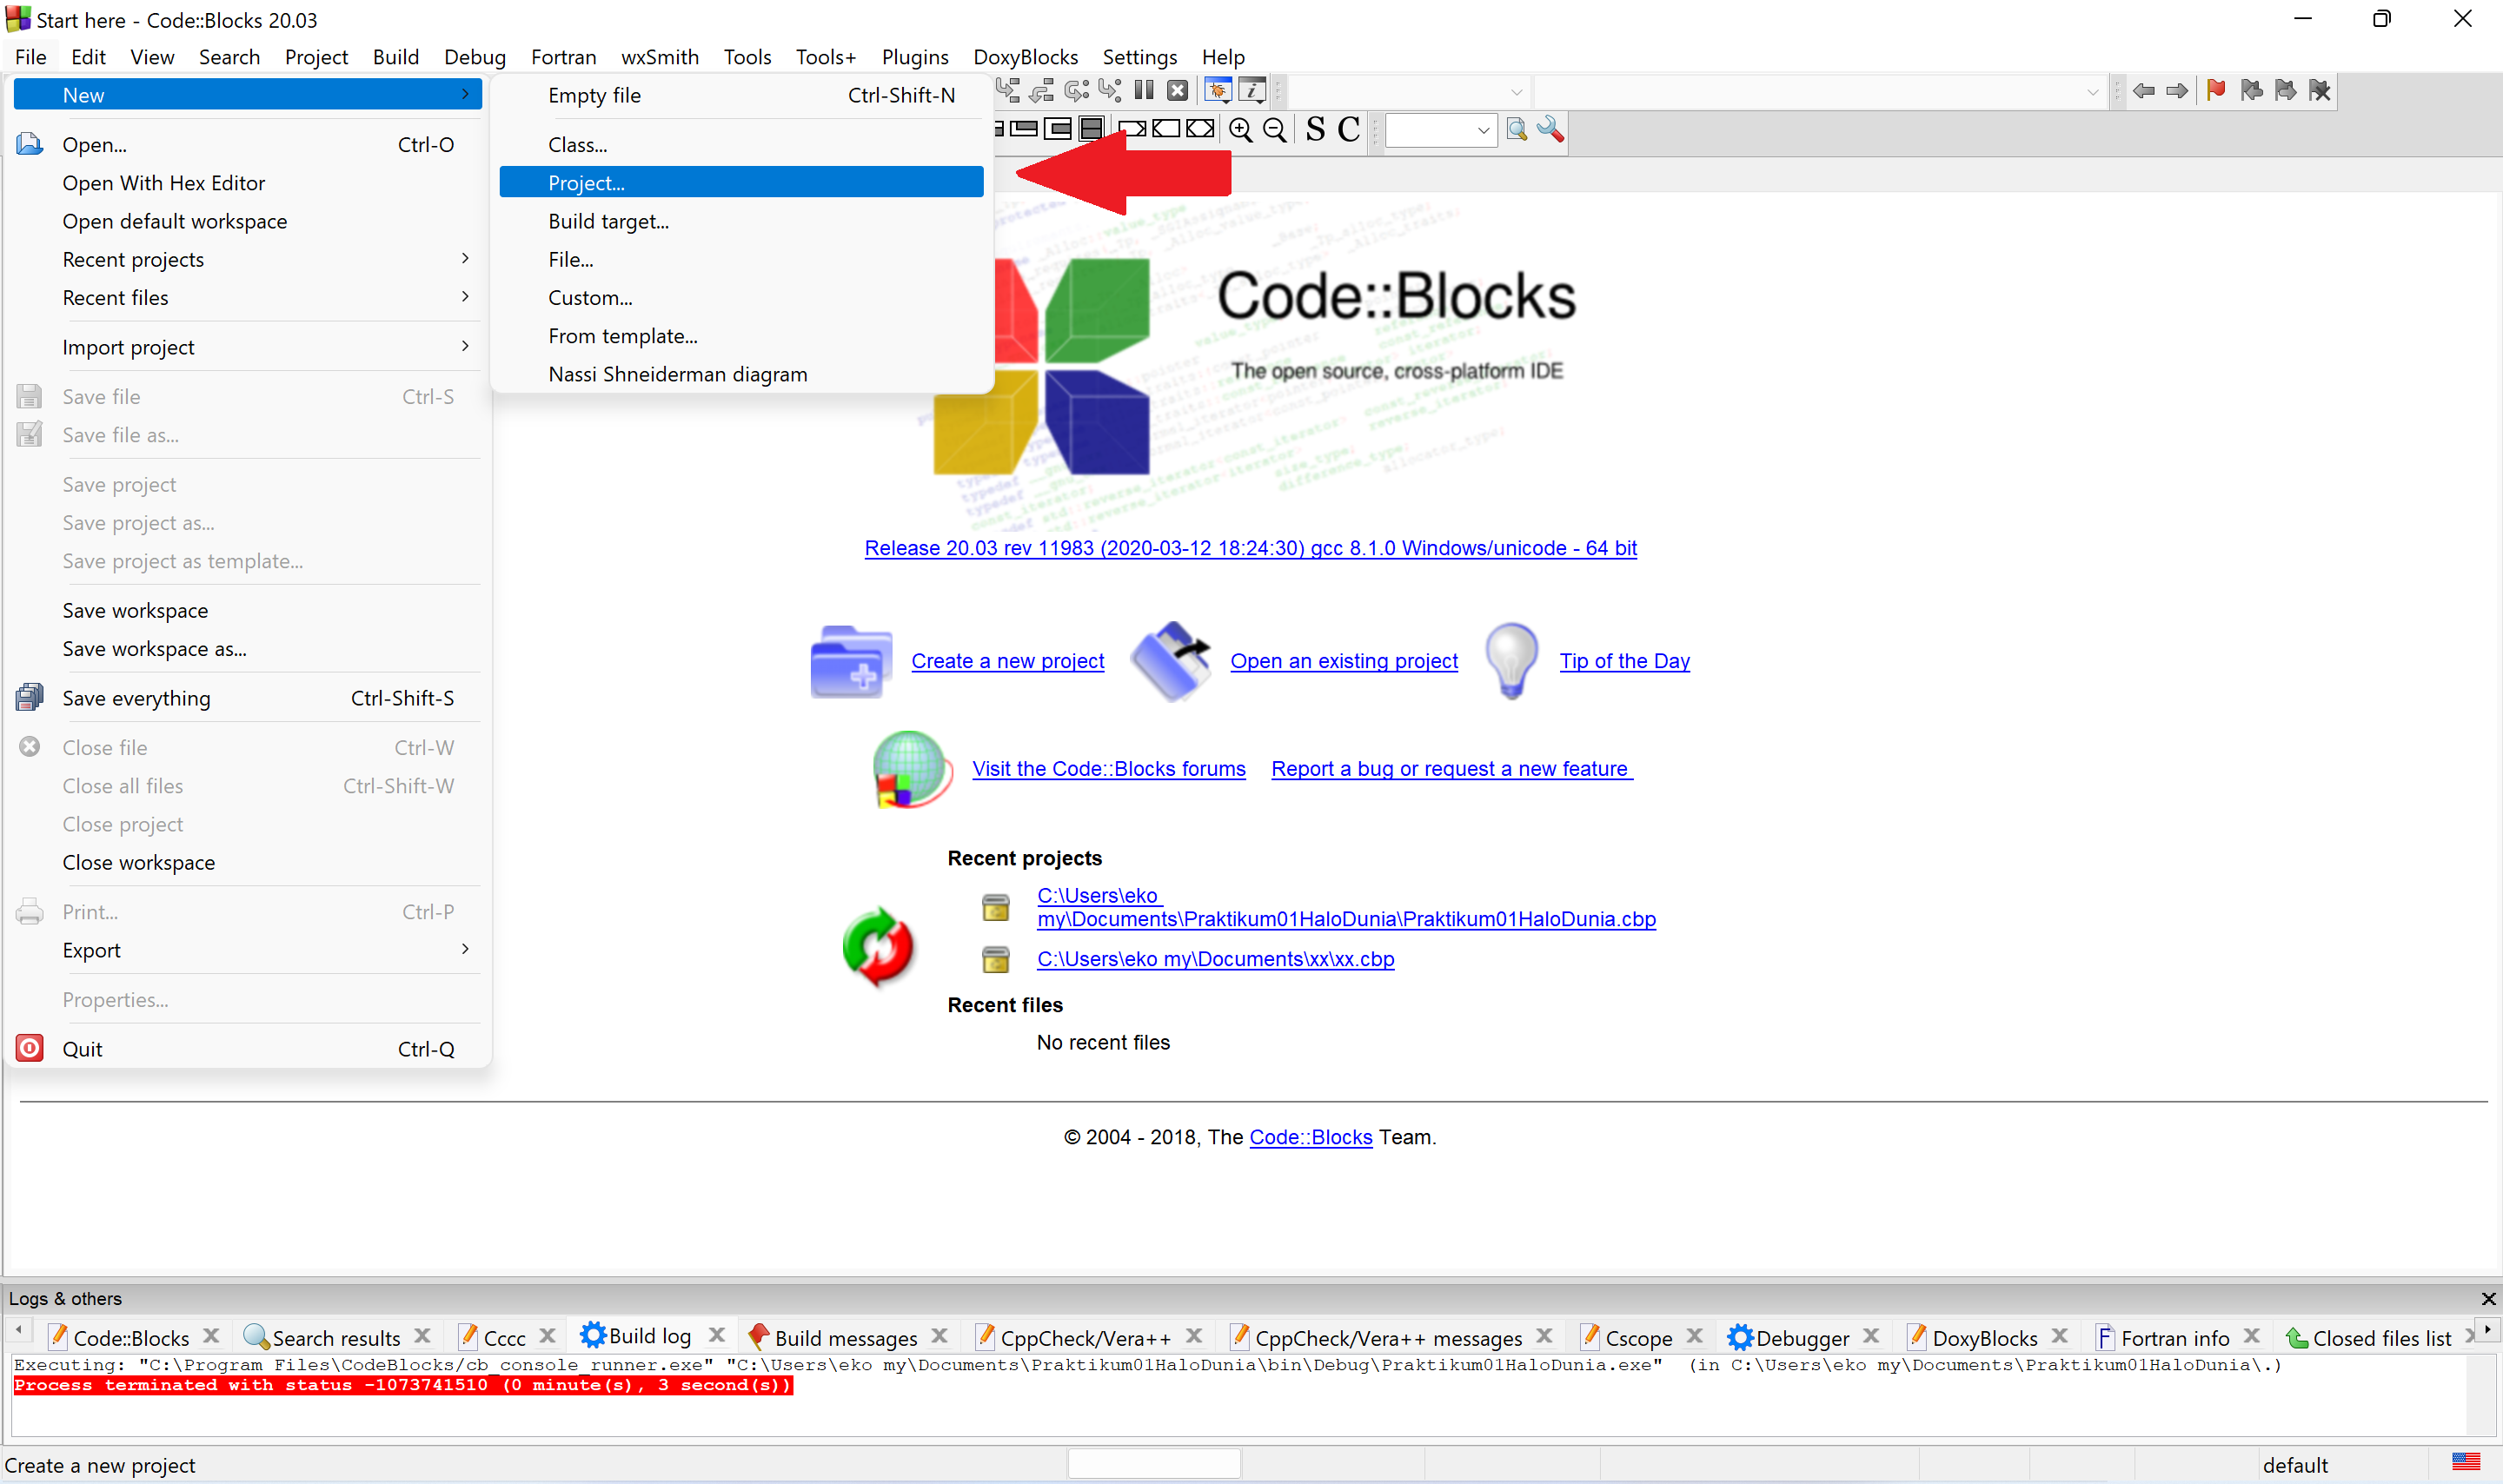
\includegraphics[width=0.7\linewidth]{P1/img/screenshot002.png}
		      \caption{}
		      \label{fig:screenshot002}
	      \end{figure}
	\item Klik Console Application
	      \begin{figure}[H]
		      \centering
		      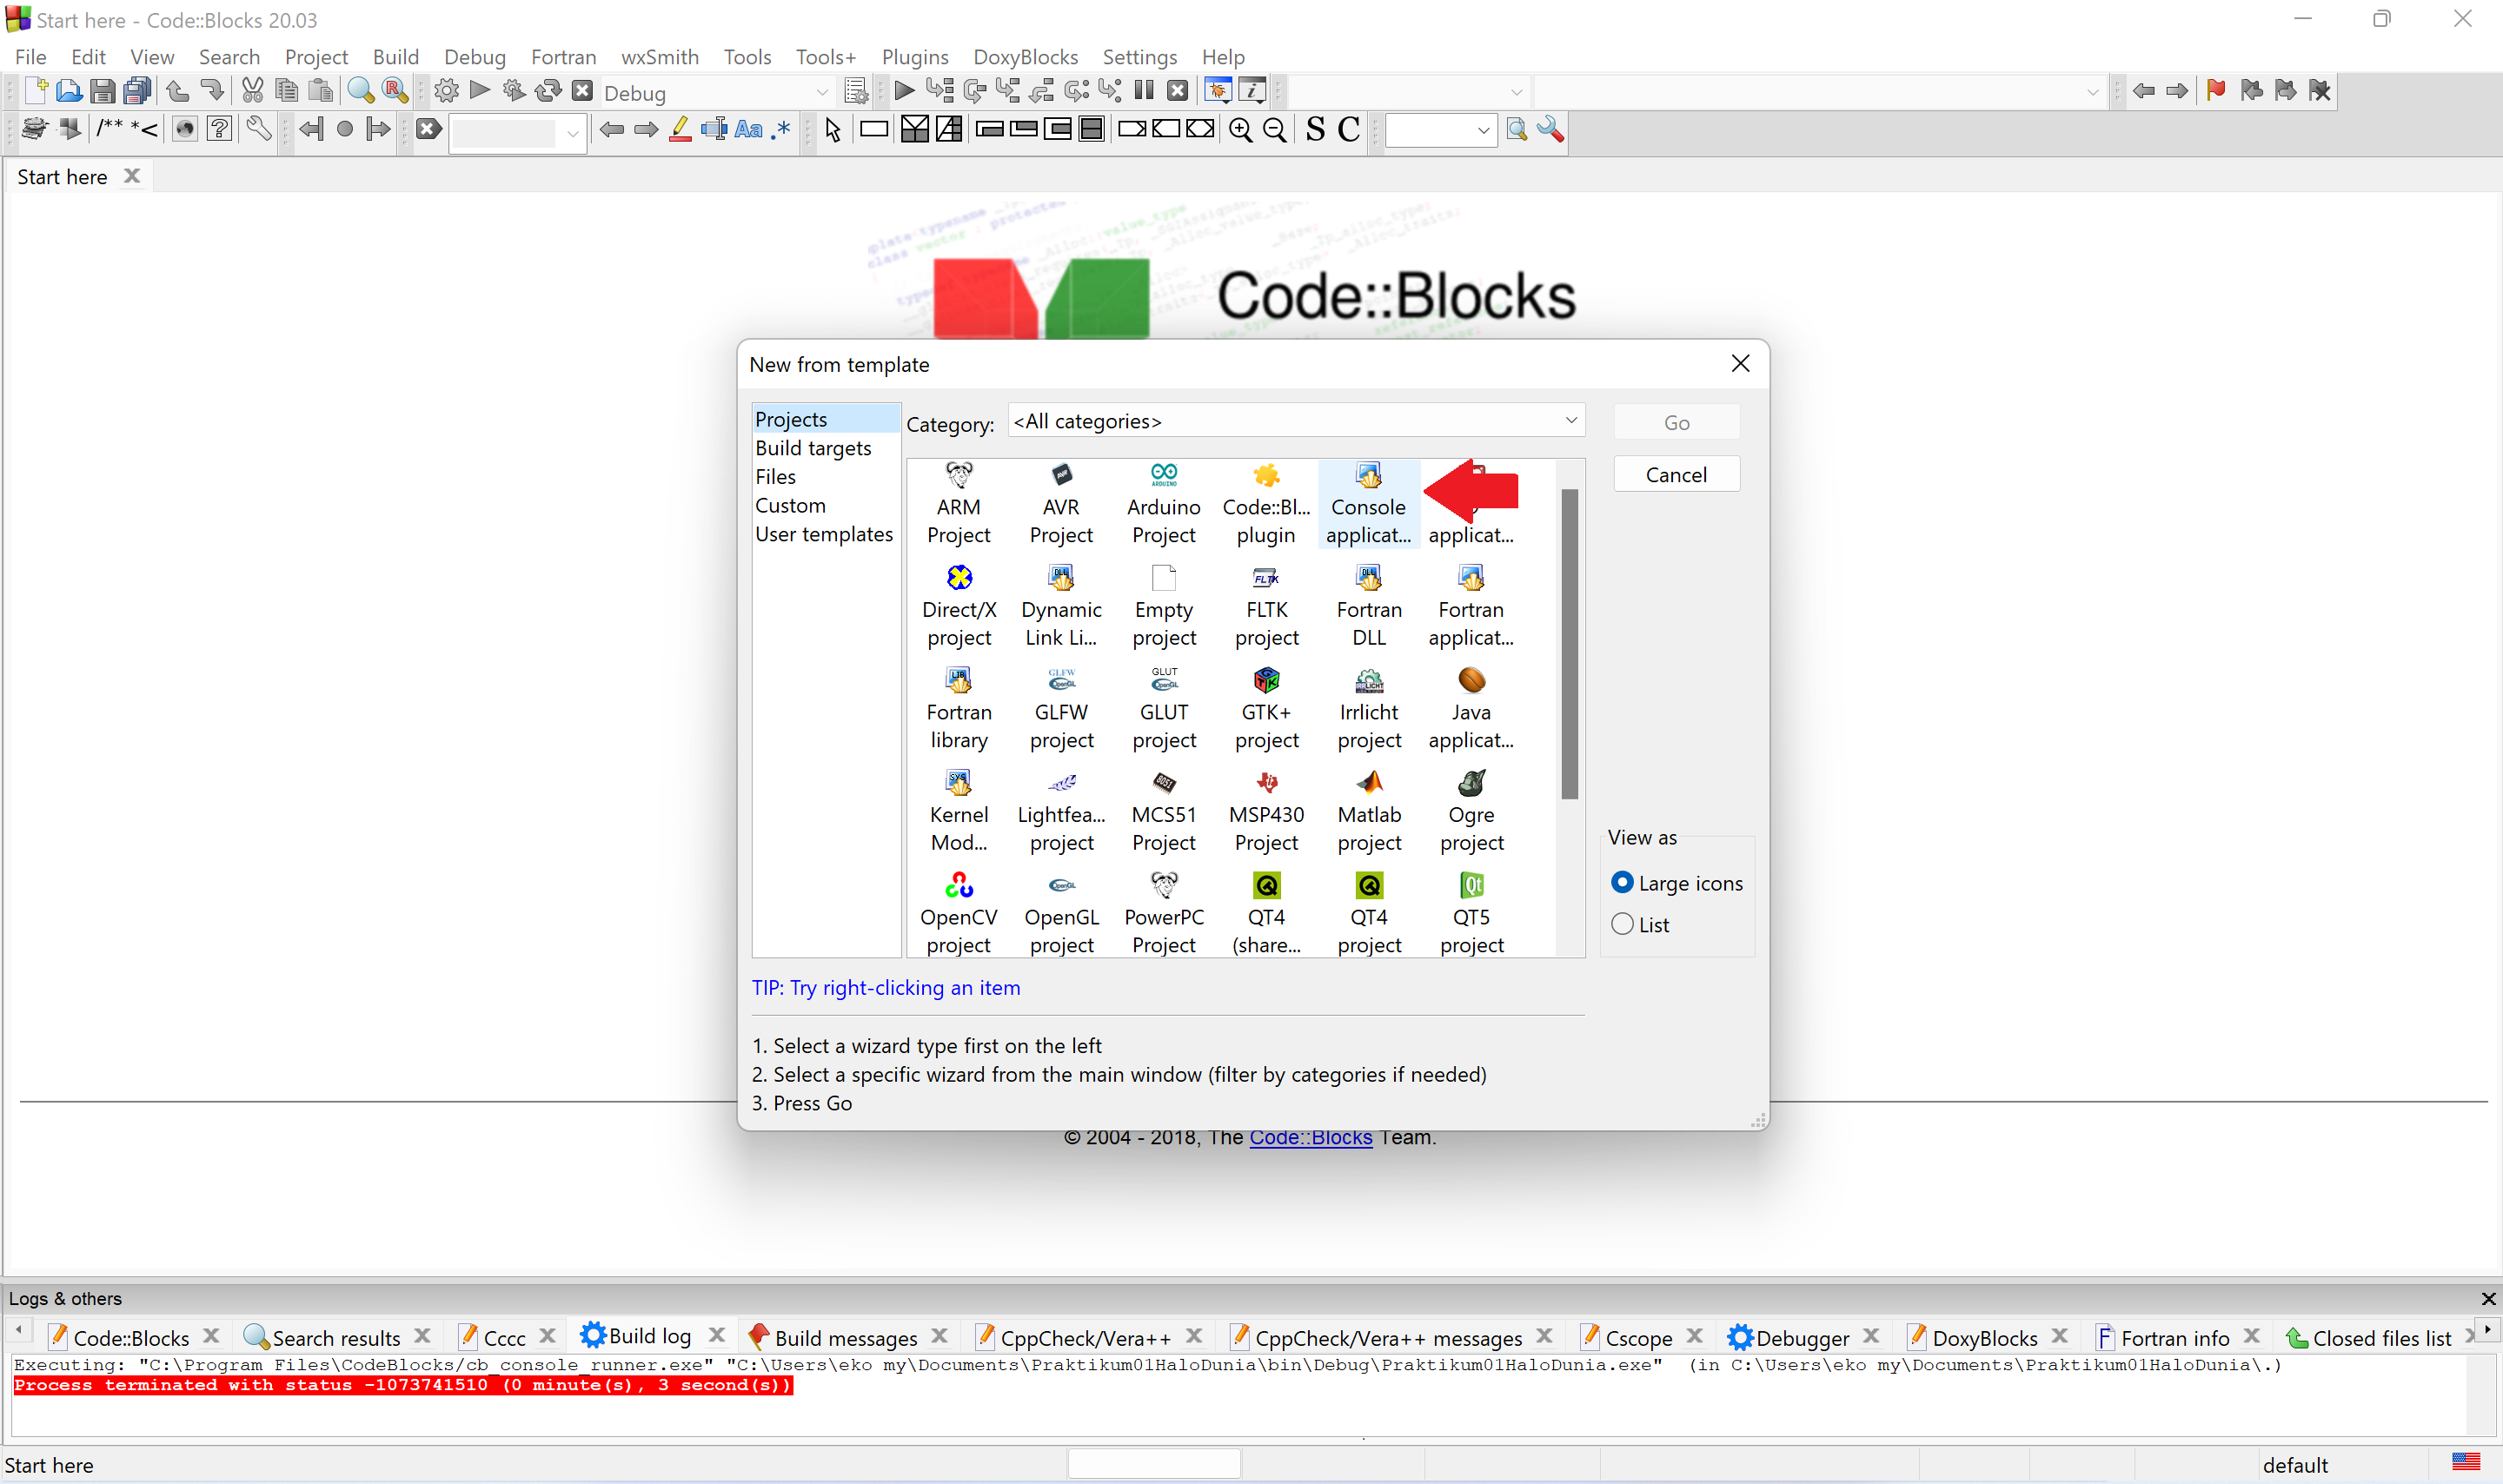
\includegraphics[width=0.7\linewidth]{P1/img/screenshot004.png}
		      \caption{}
		      \label{fig:screenshot004}
	      \end{figure}
	\item Pilih C sebagai bahasa Pemrograman
	      \begin{figure}[H]
		      \centering
		      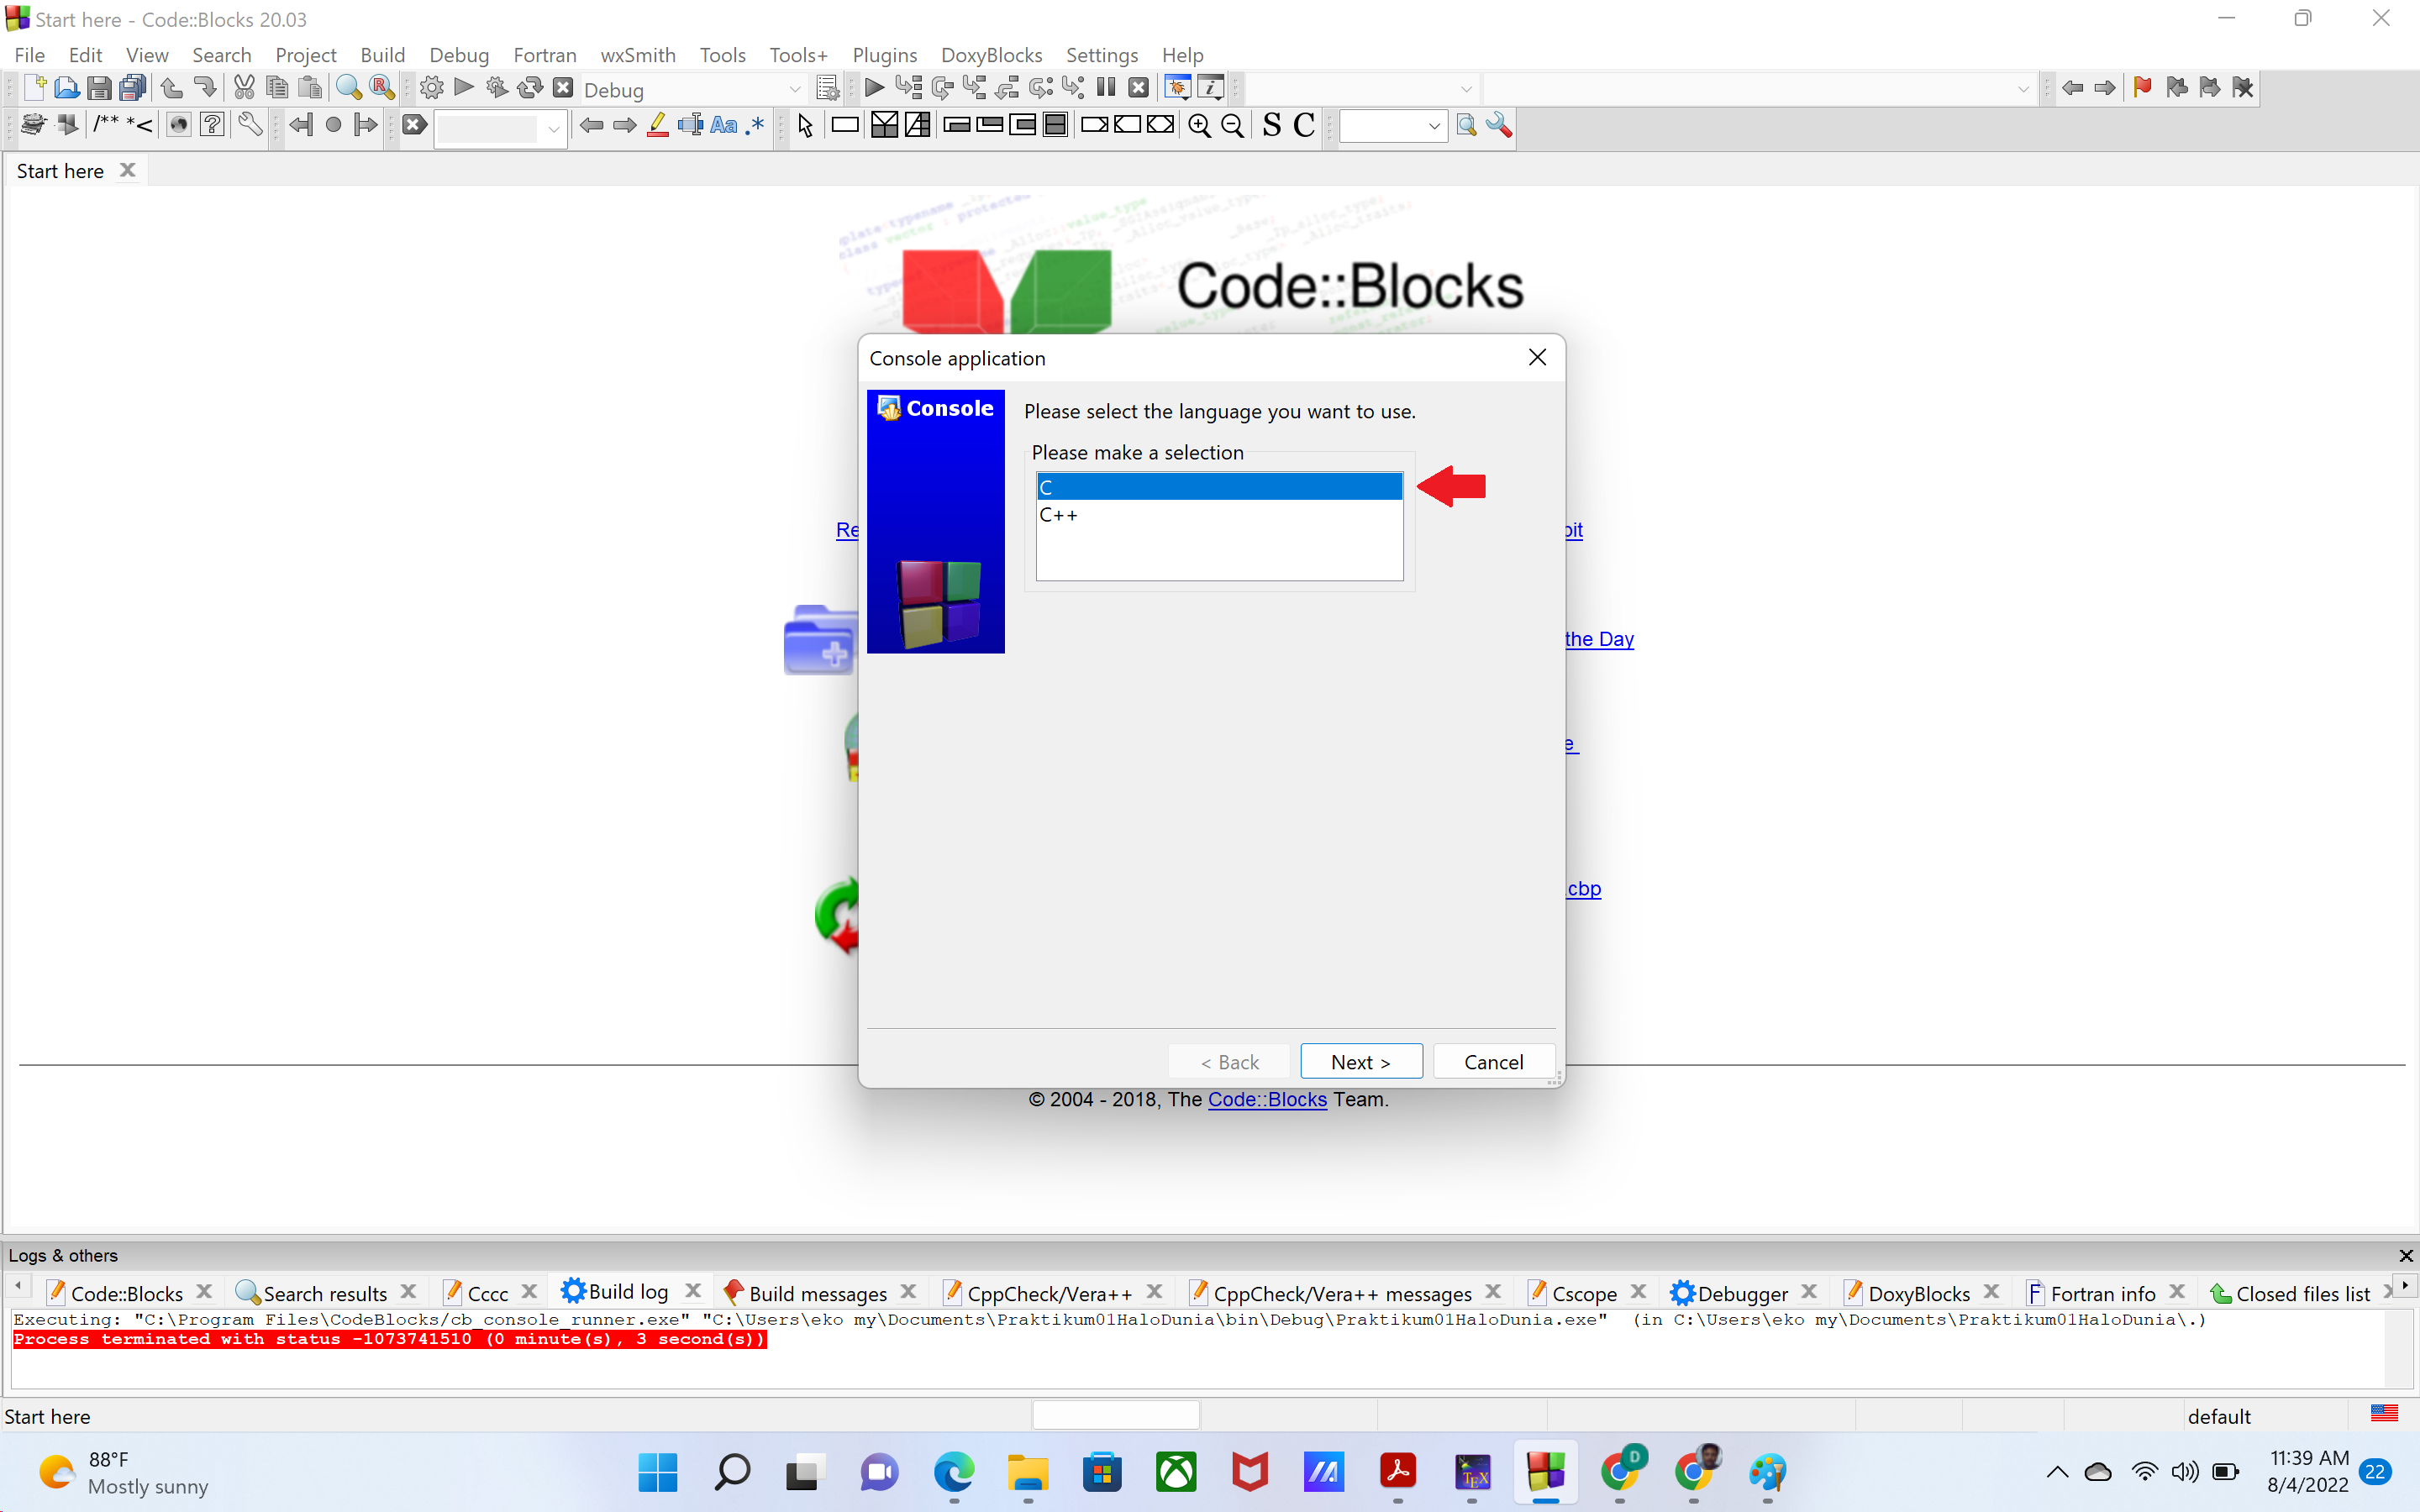
\includegraphics[width=0.7\linewidth]{P1/img/screenshot005.png}
		      \caption{}
		      \label{fig:screenshot005}
	      \end{figure}
	\item Berikan nama ke project
	      \begin{figure}[H]
		      \centering
		      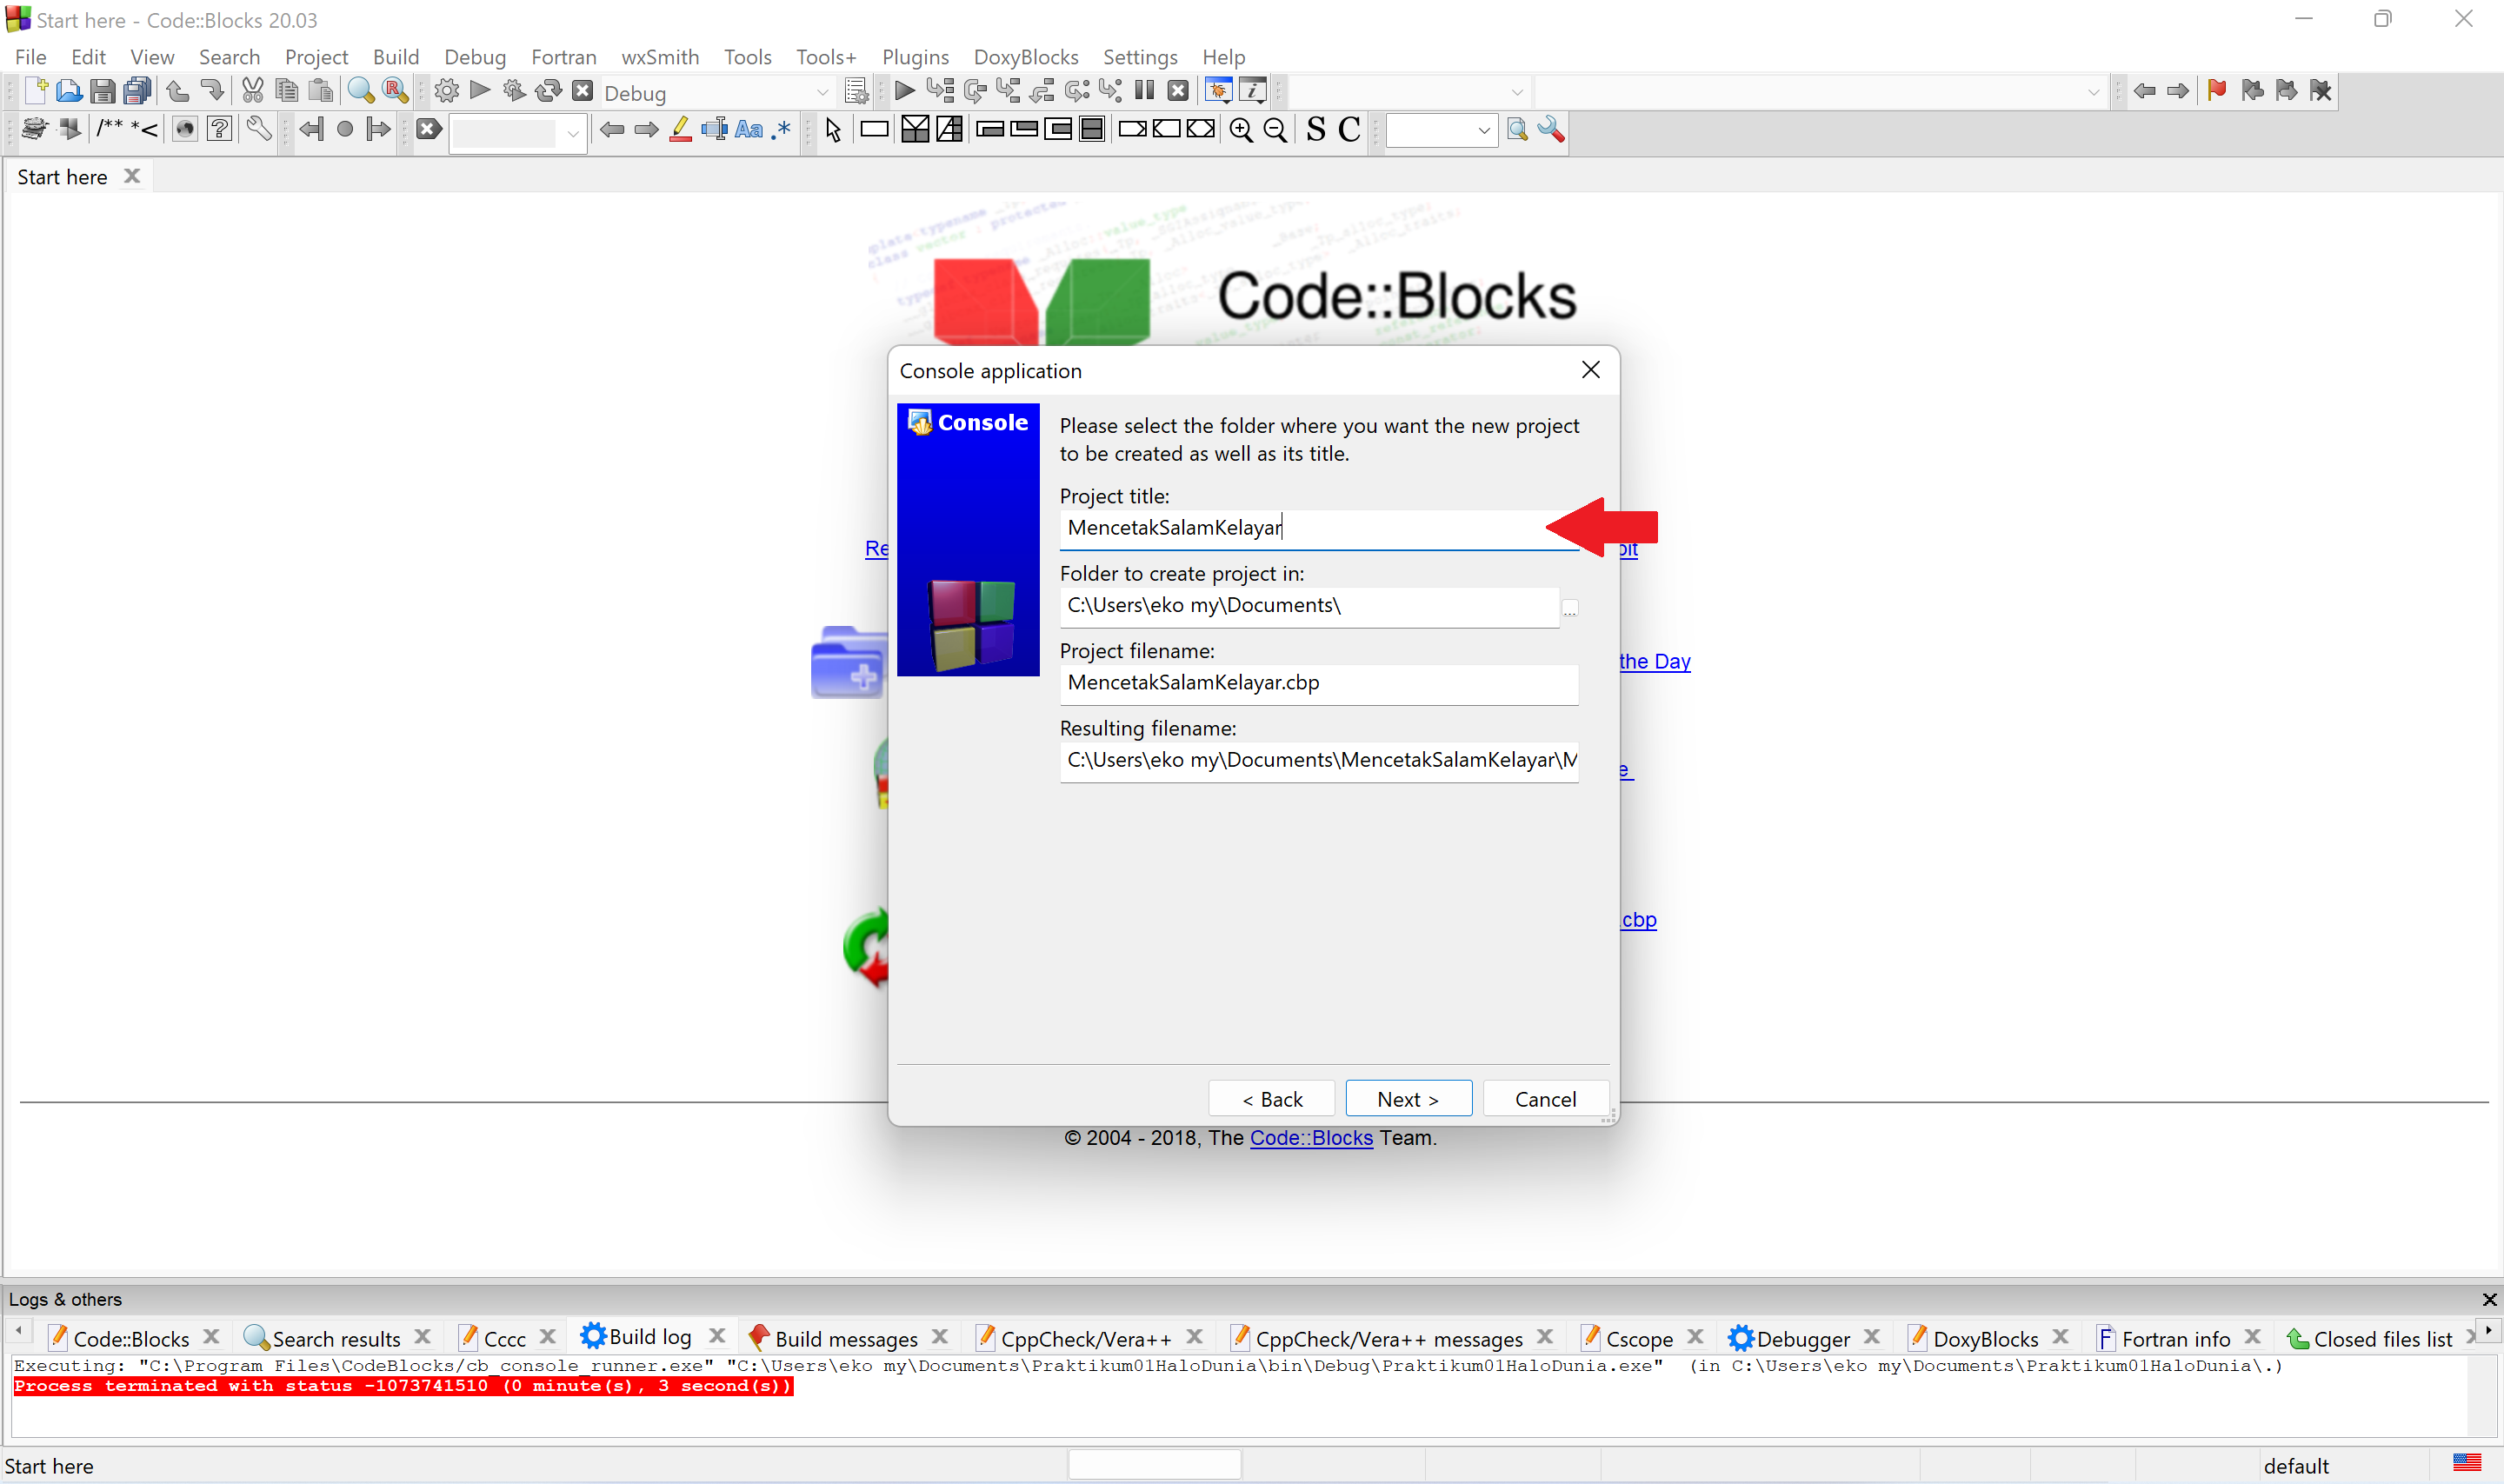
\includegraphics[width=0.7\linewidth]{P1/img/screenshot006.png}
		      \caption{}
		      \label{fig:screenshot006}
	      \end{figure}
	\item  Pilih compiler (gcc), pilih direktori untuk menyimpan, dan klik save.
	      \begin{figure}[H]
		      \centering
		      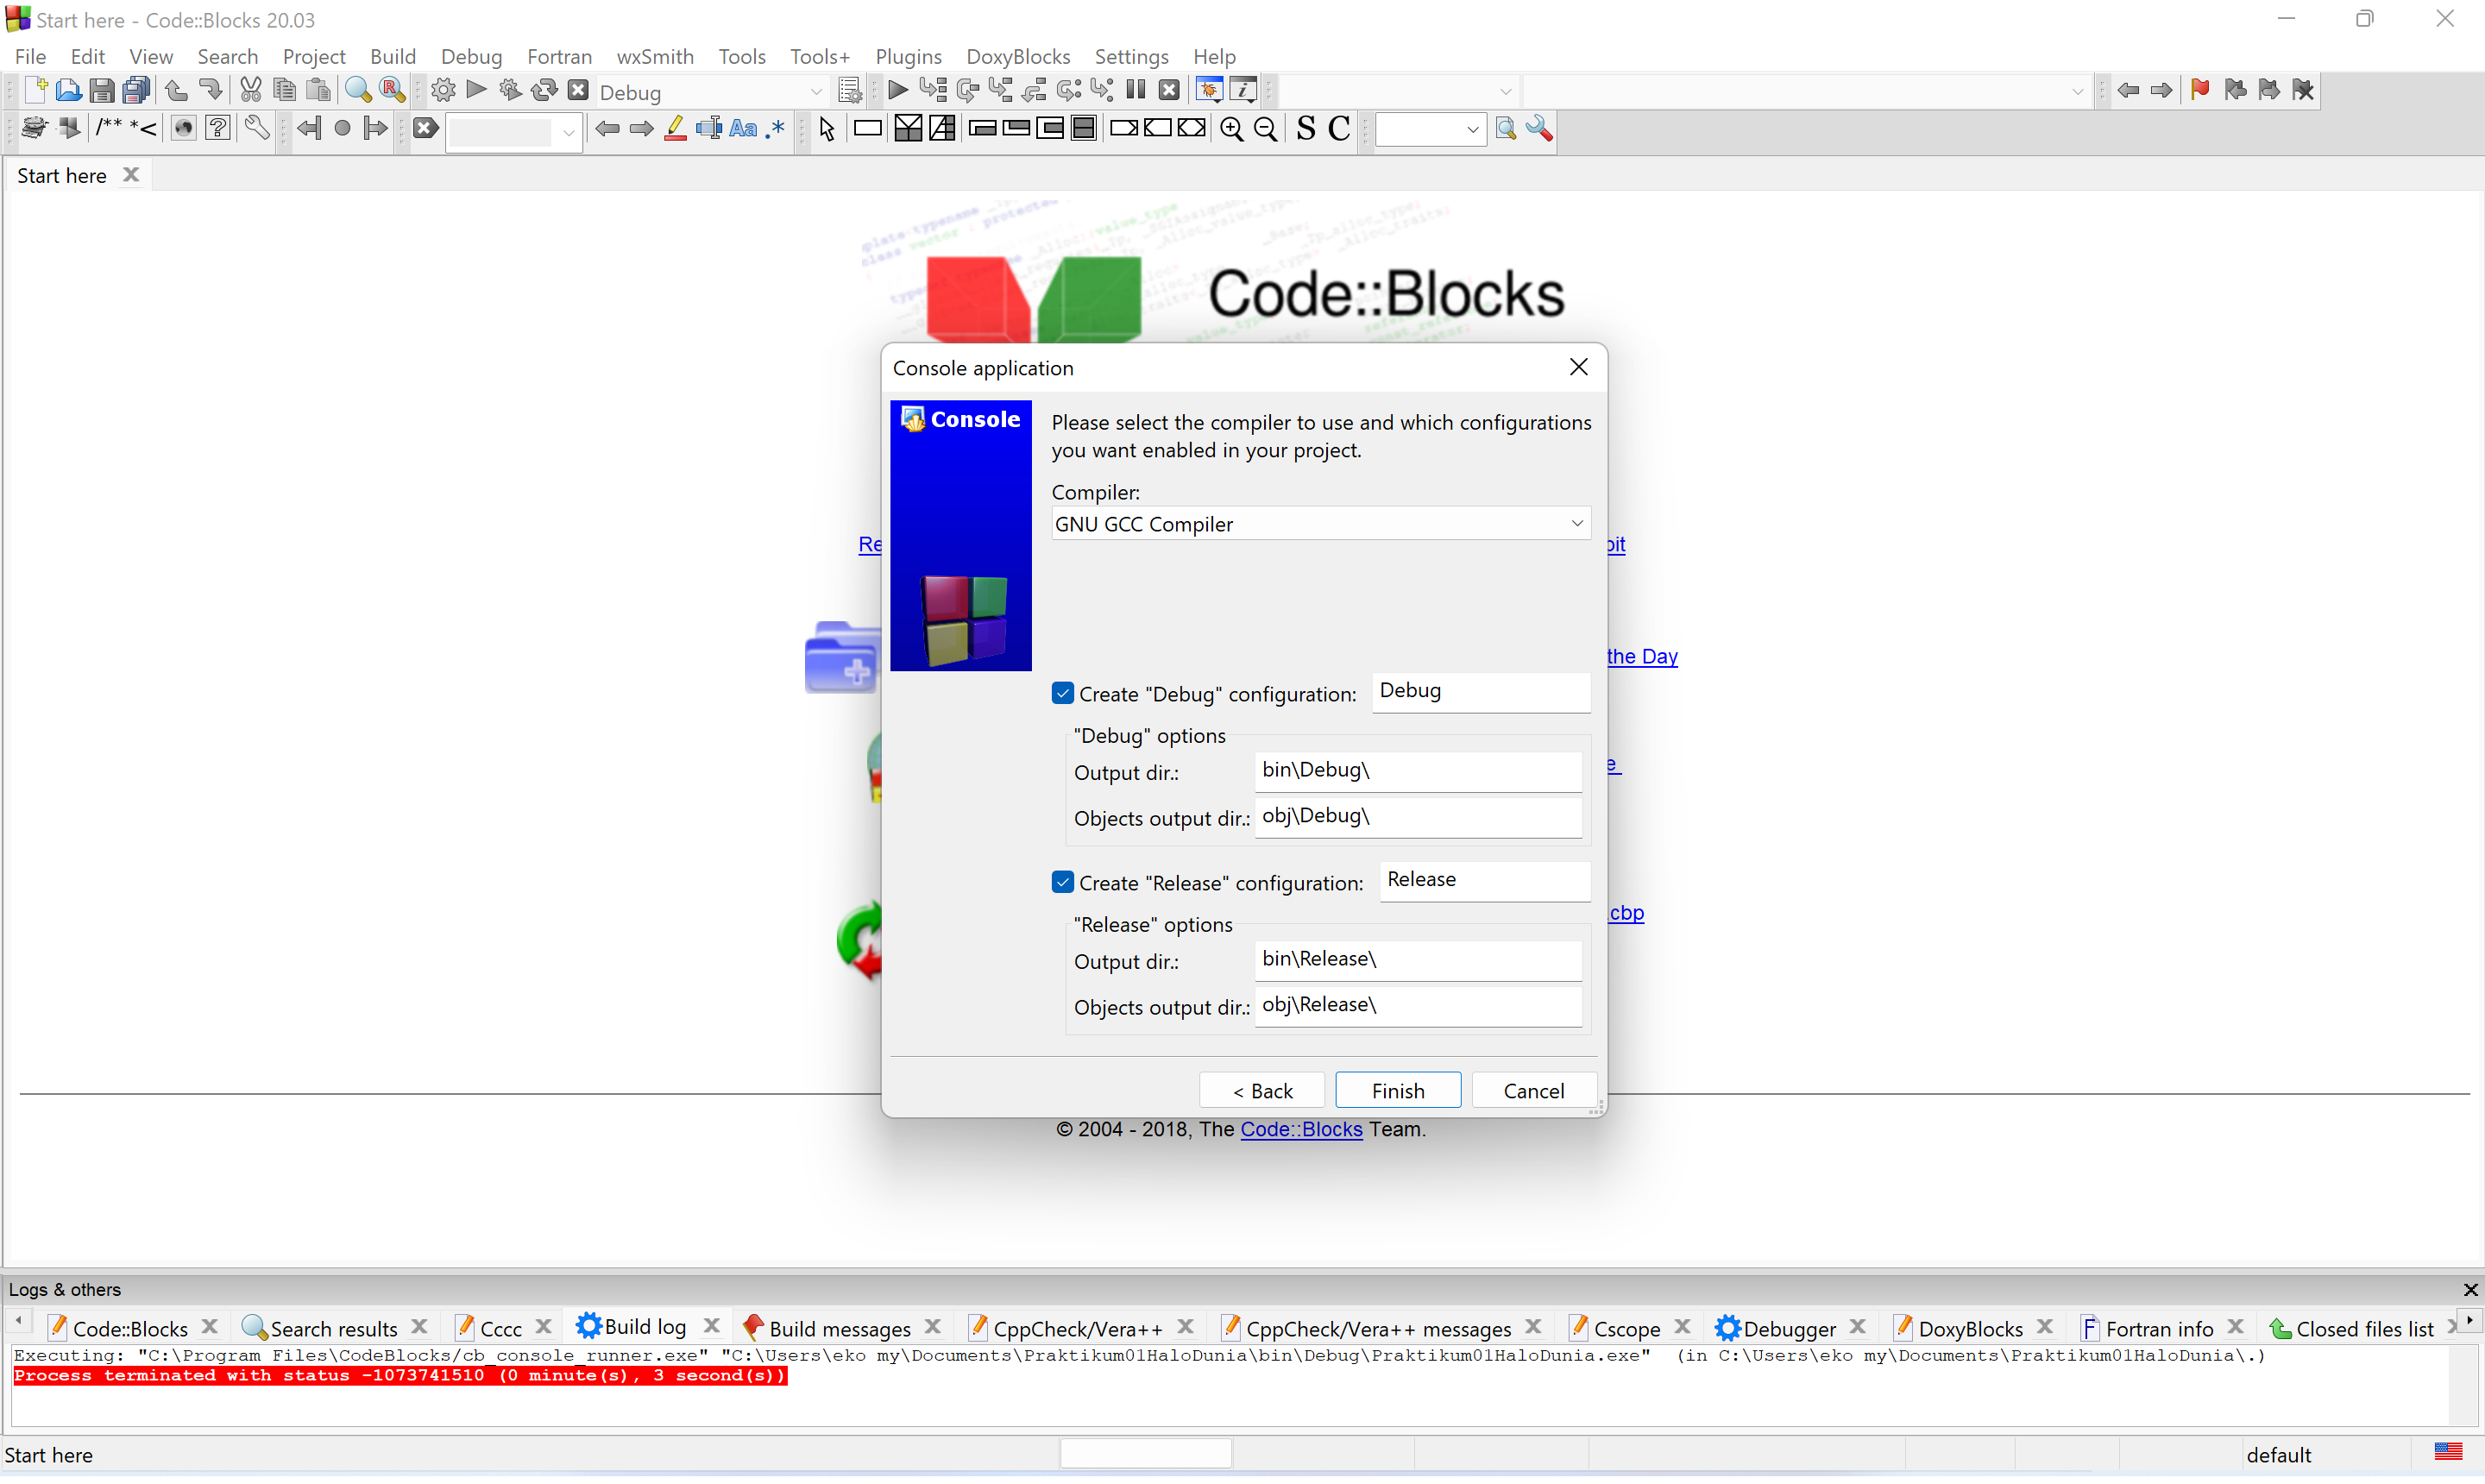
\includegraphics[width=0.7\linewidth]{P1/img/screenshot007.png}
		      \caption{}
		      \label{fig:screenshot007}
	      \end{figure}
	\item Ketikan kode pada Gambar\ref{fig:screenshot008} ke Code::Blocks
	      \begin{figure}[H]
		      \centering
		      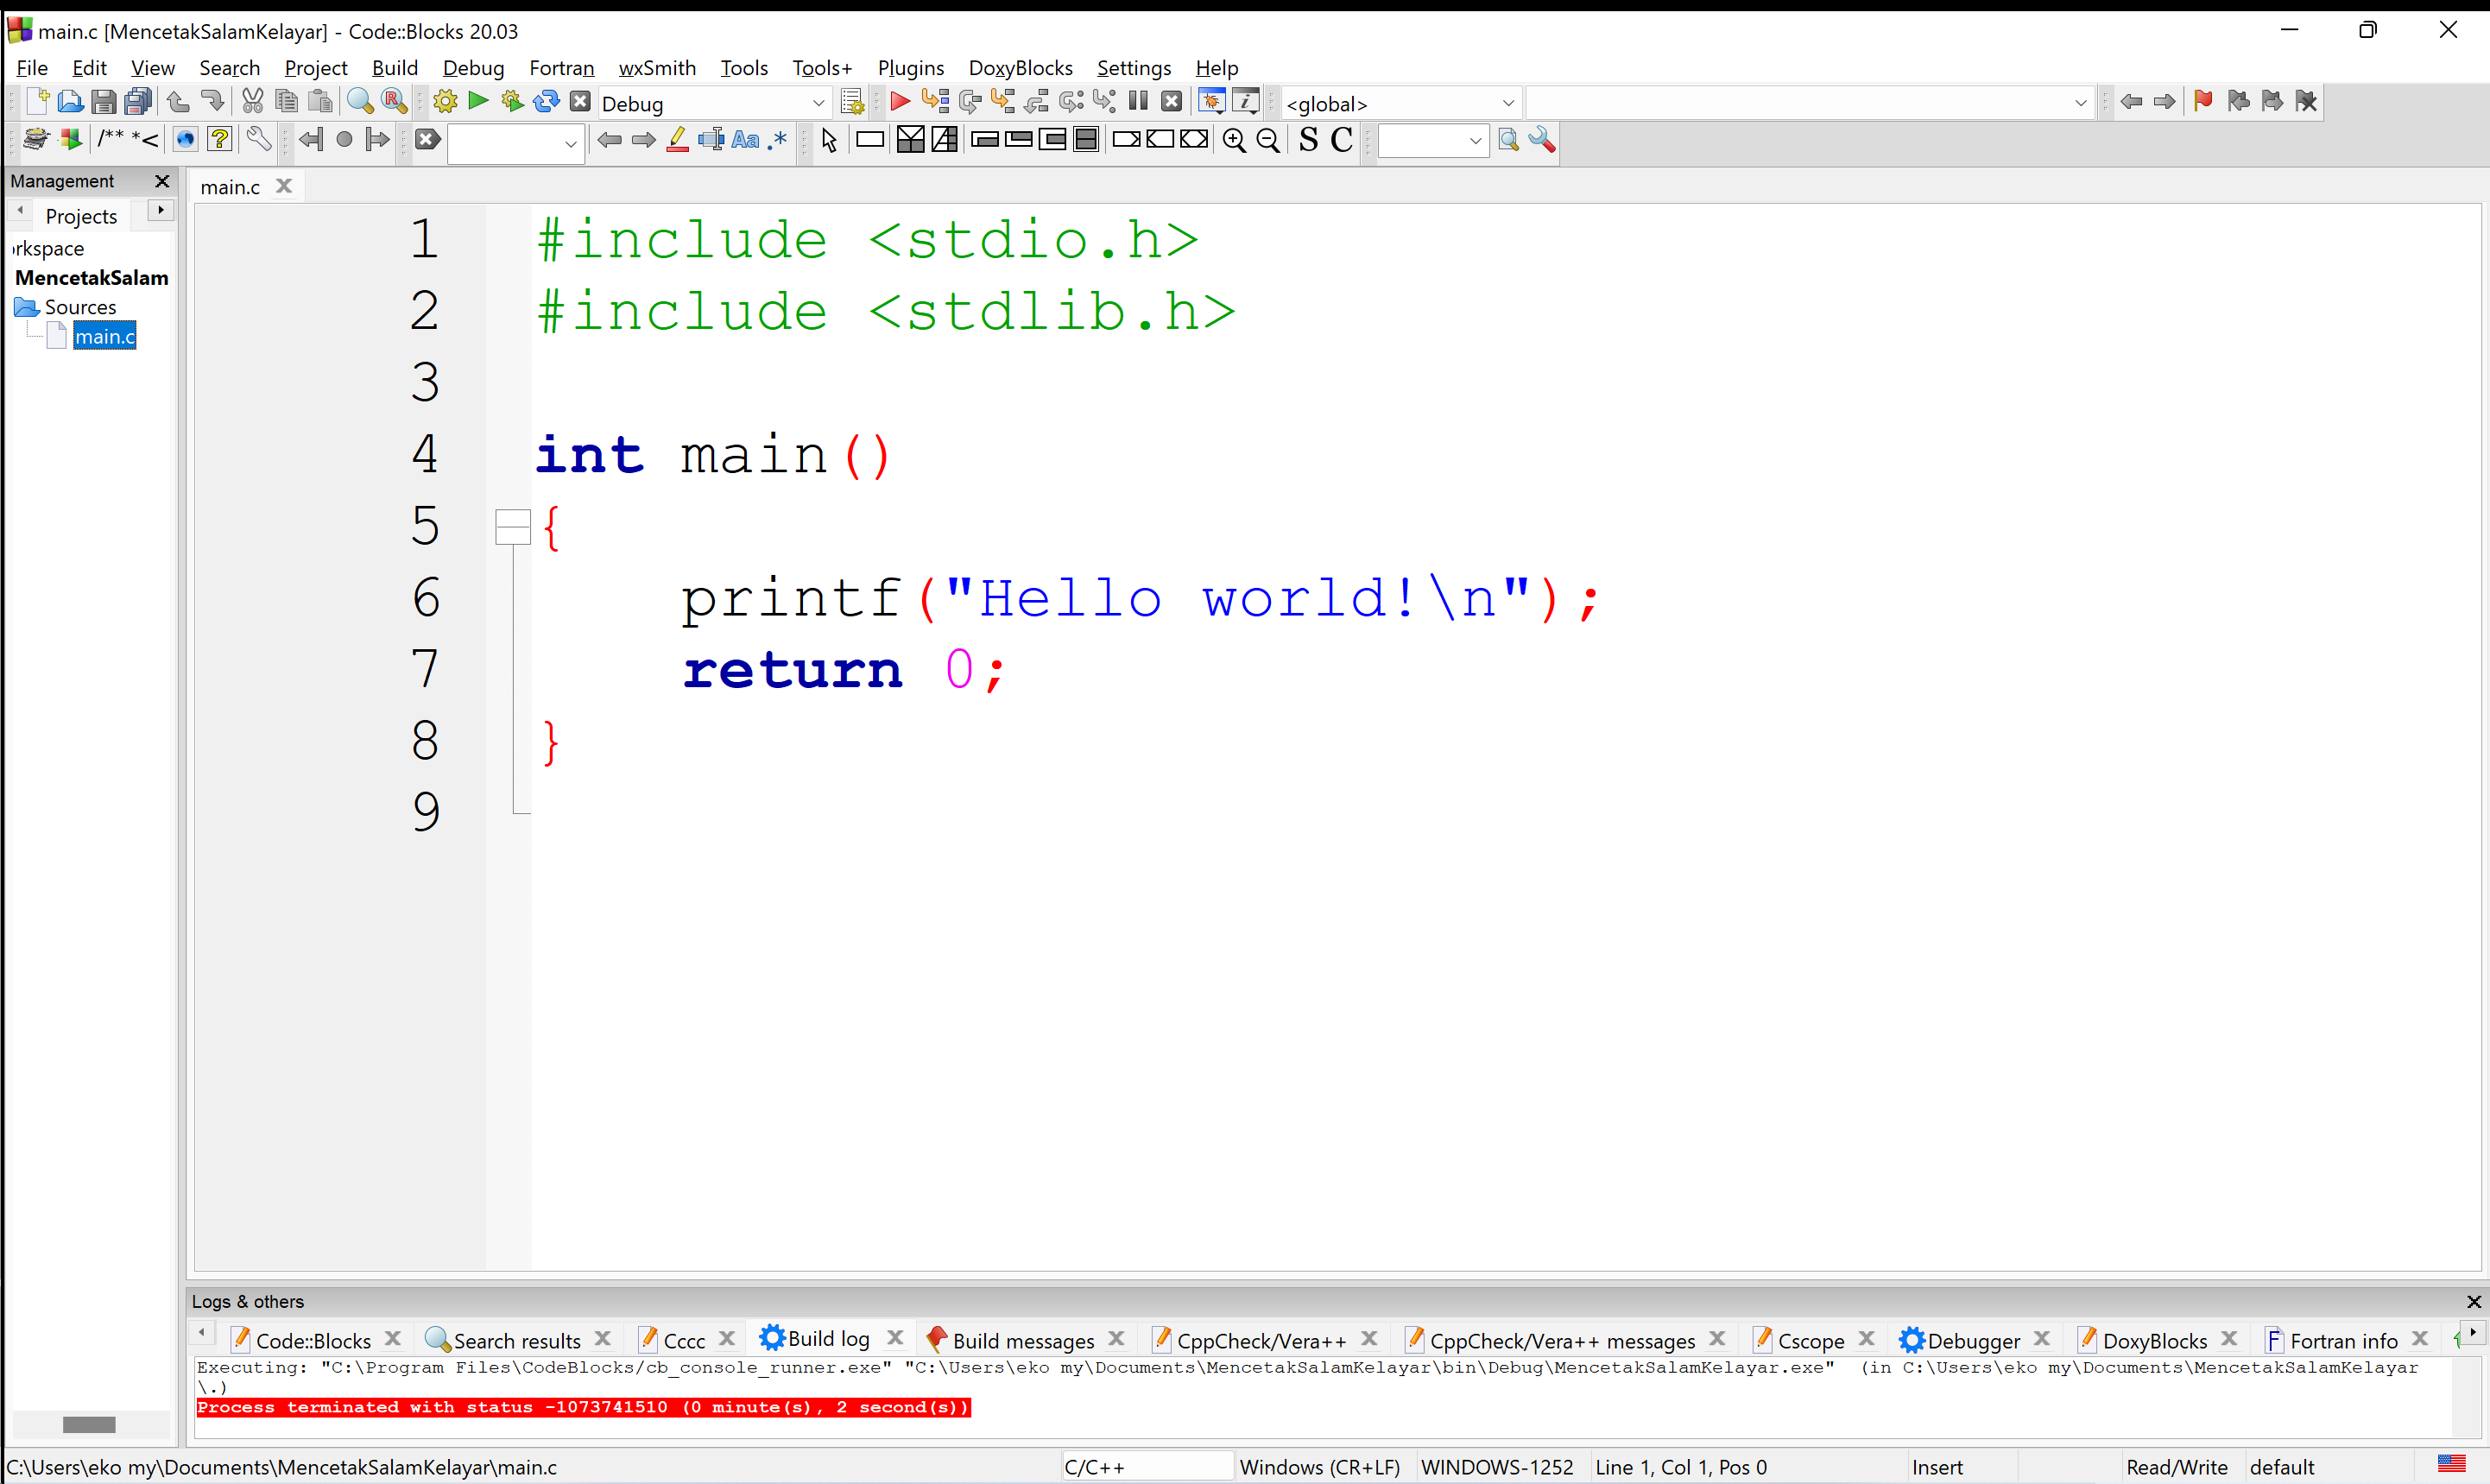
\includegraphics[width=0.7\linewidth]{P1/img/screenshot008.png}
		      \caption{}
		      \label{fig:screenshot008}
	      \end{figure}
	\item Klik Build$->$Build and Run atau tekan F9
	      \begin{figure}[H]
		      \centering
		      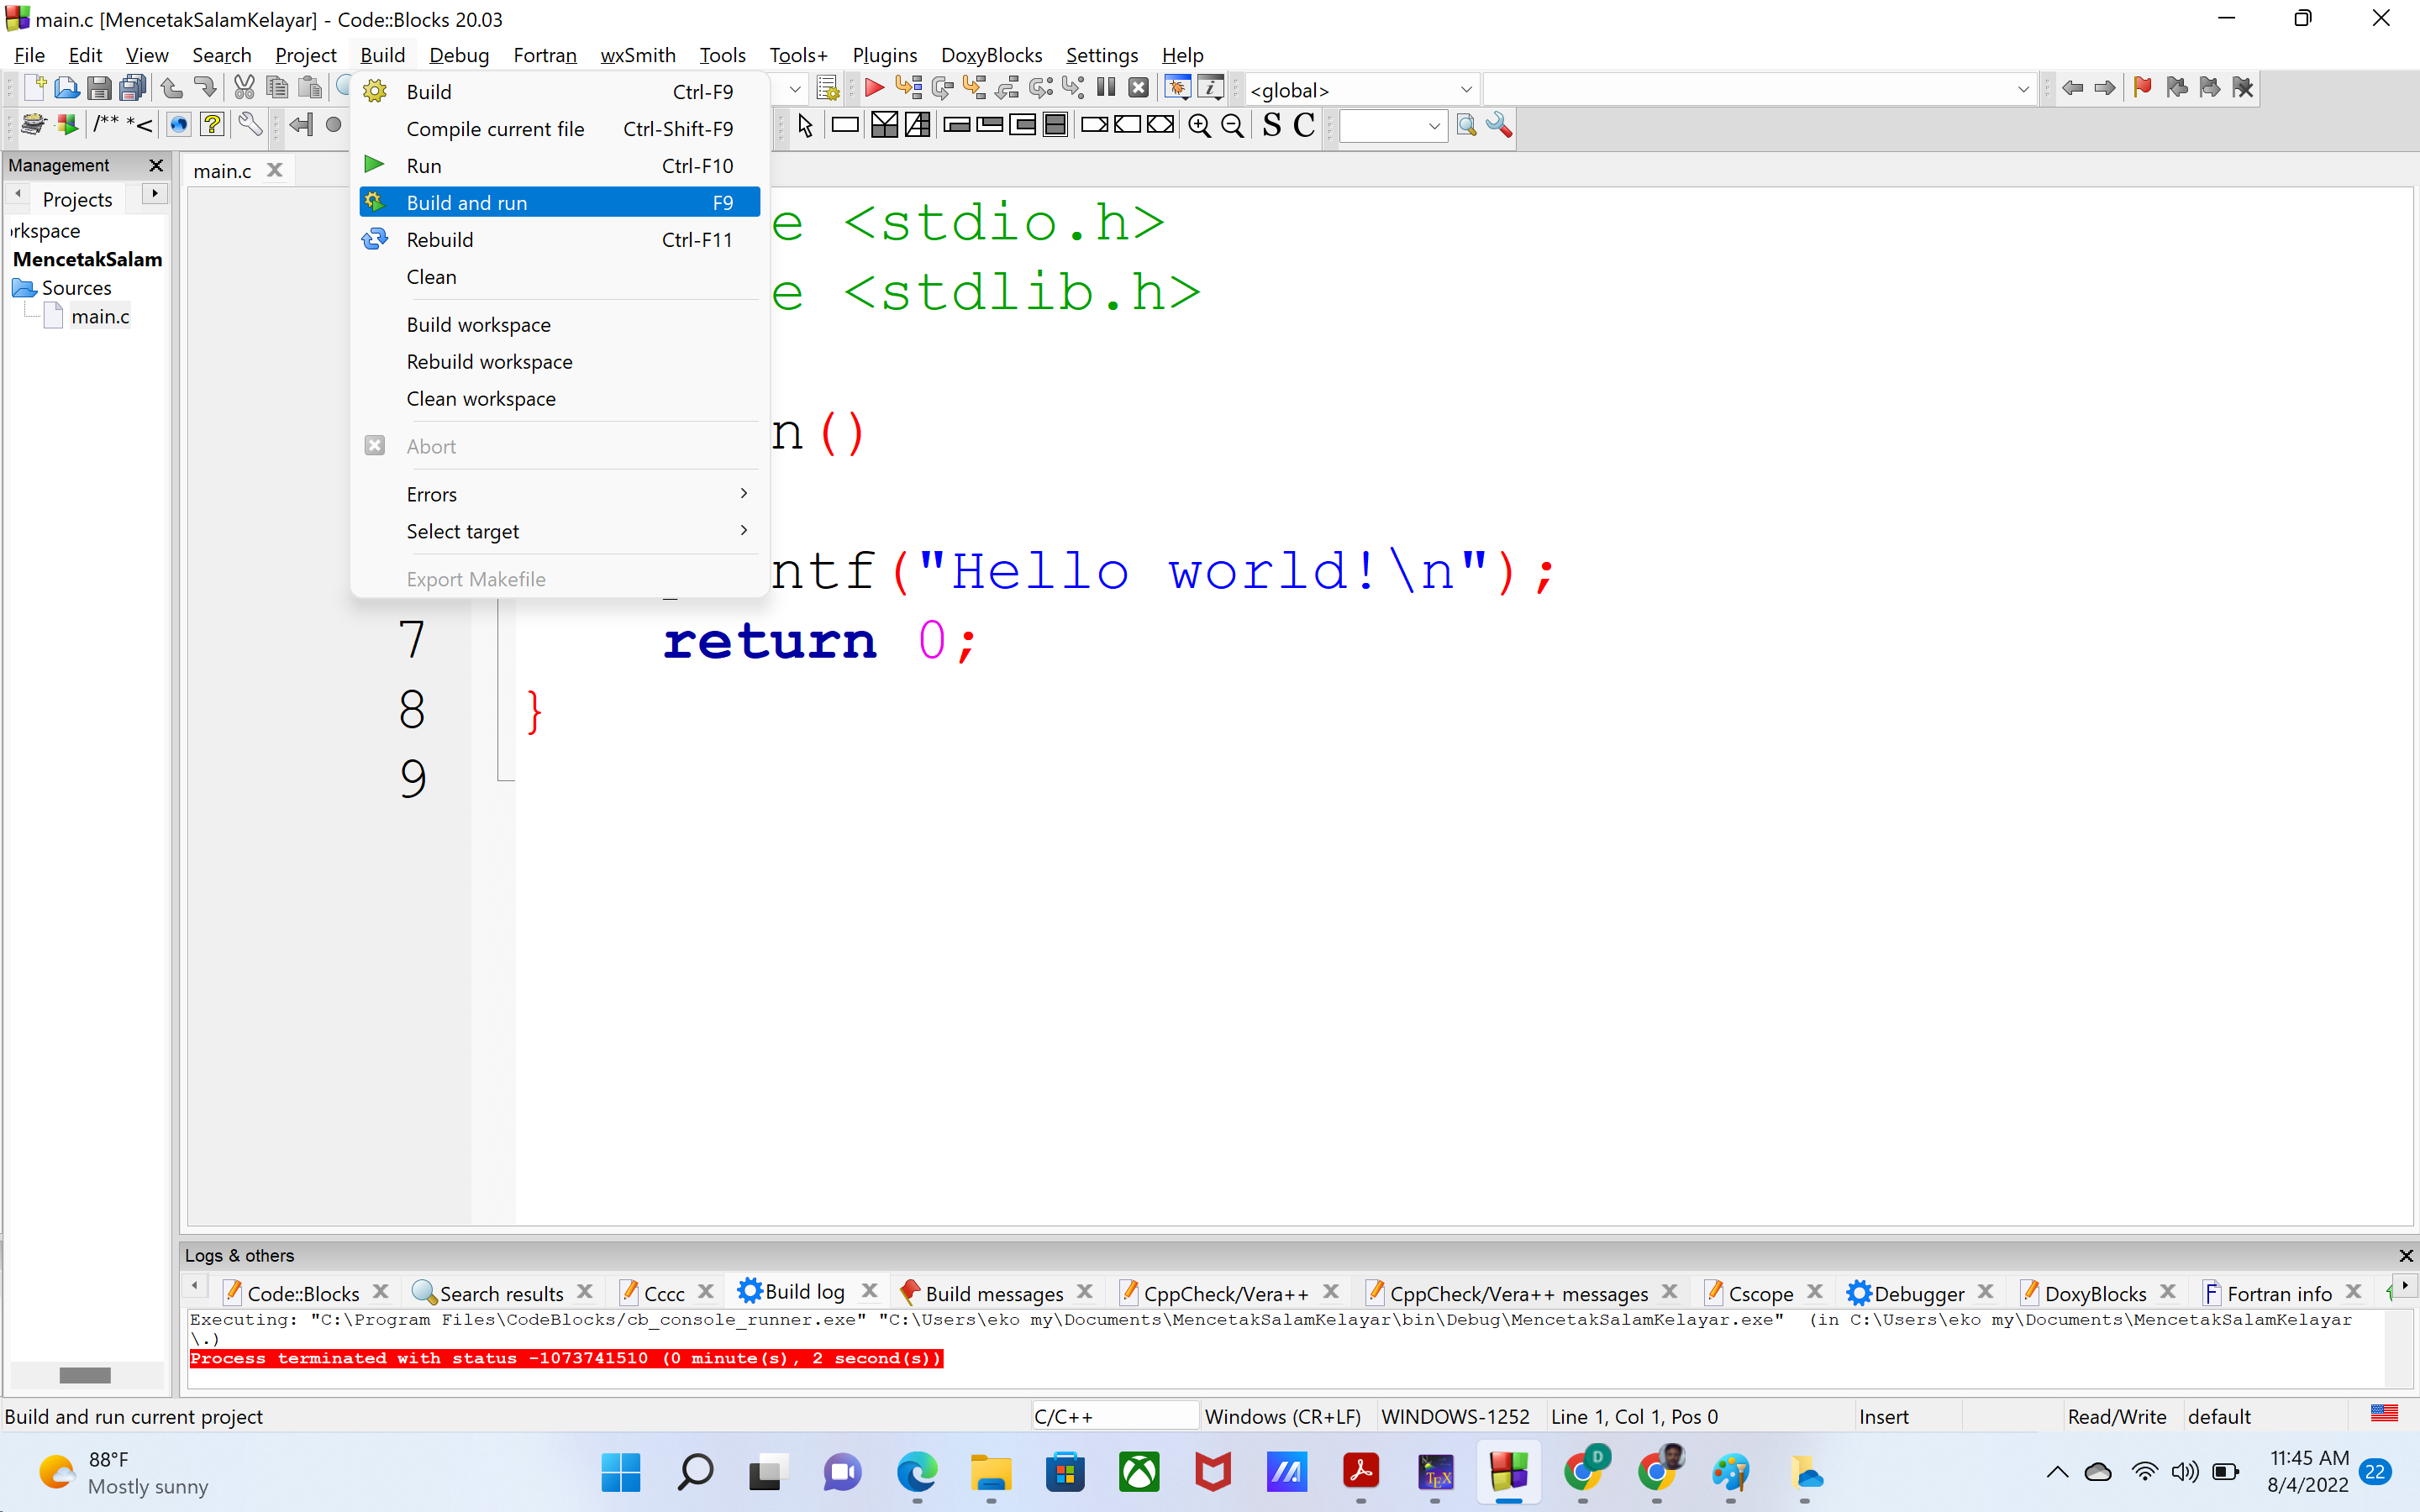
\includegraphics[width=0.7\linewidth]{P1/img/screenshot009.png}
		      \caption{}
		      \label{fig:screenshot009}
	      \end{figure}
	\item Keluaran dari program dapat dilihat di console
	      \begin{figure}[H]
		      \centering
		      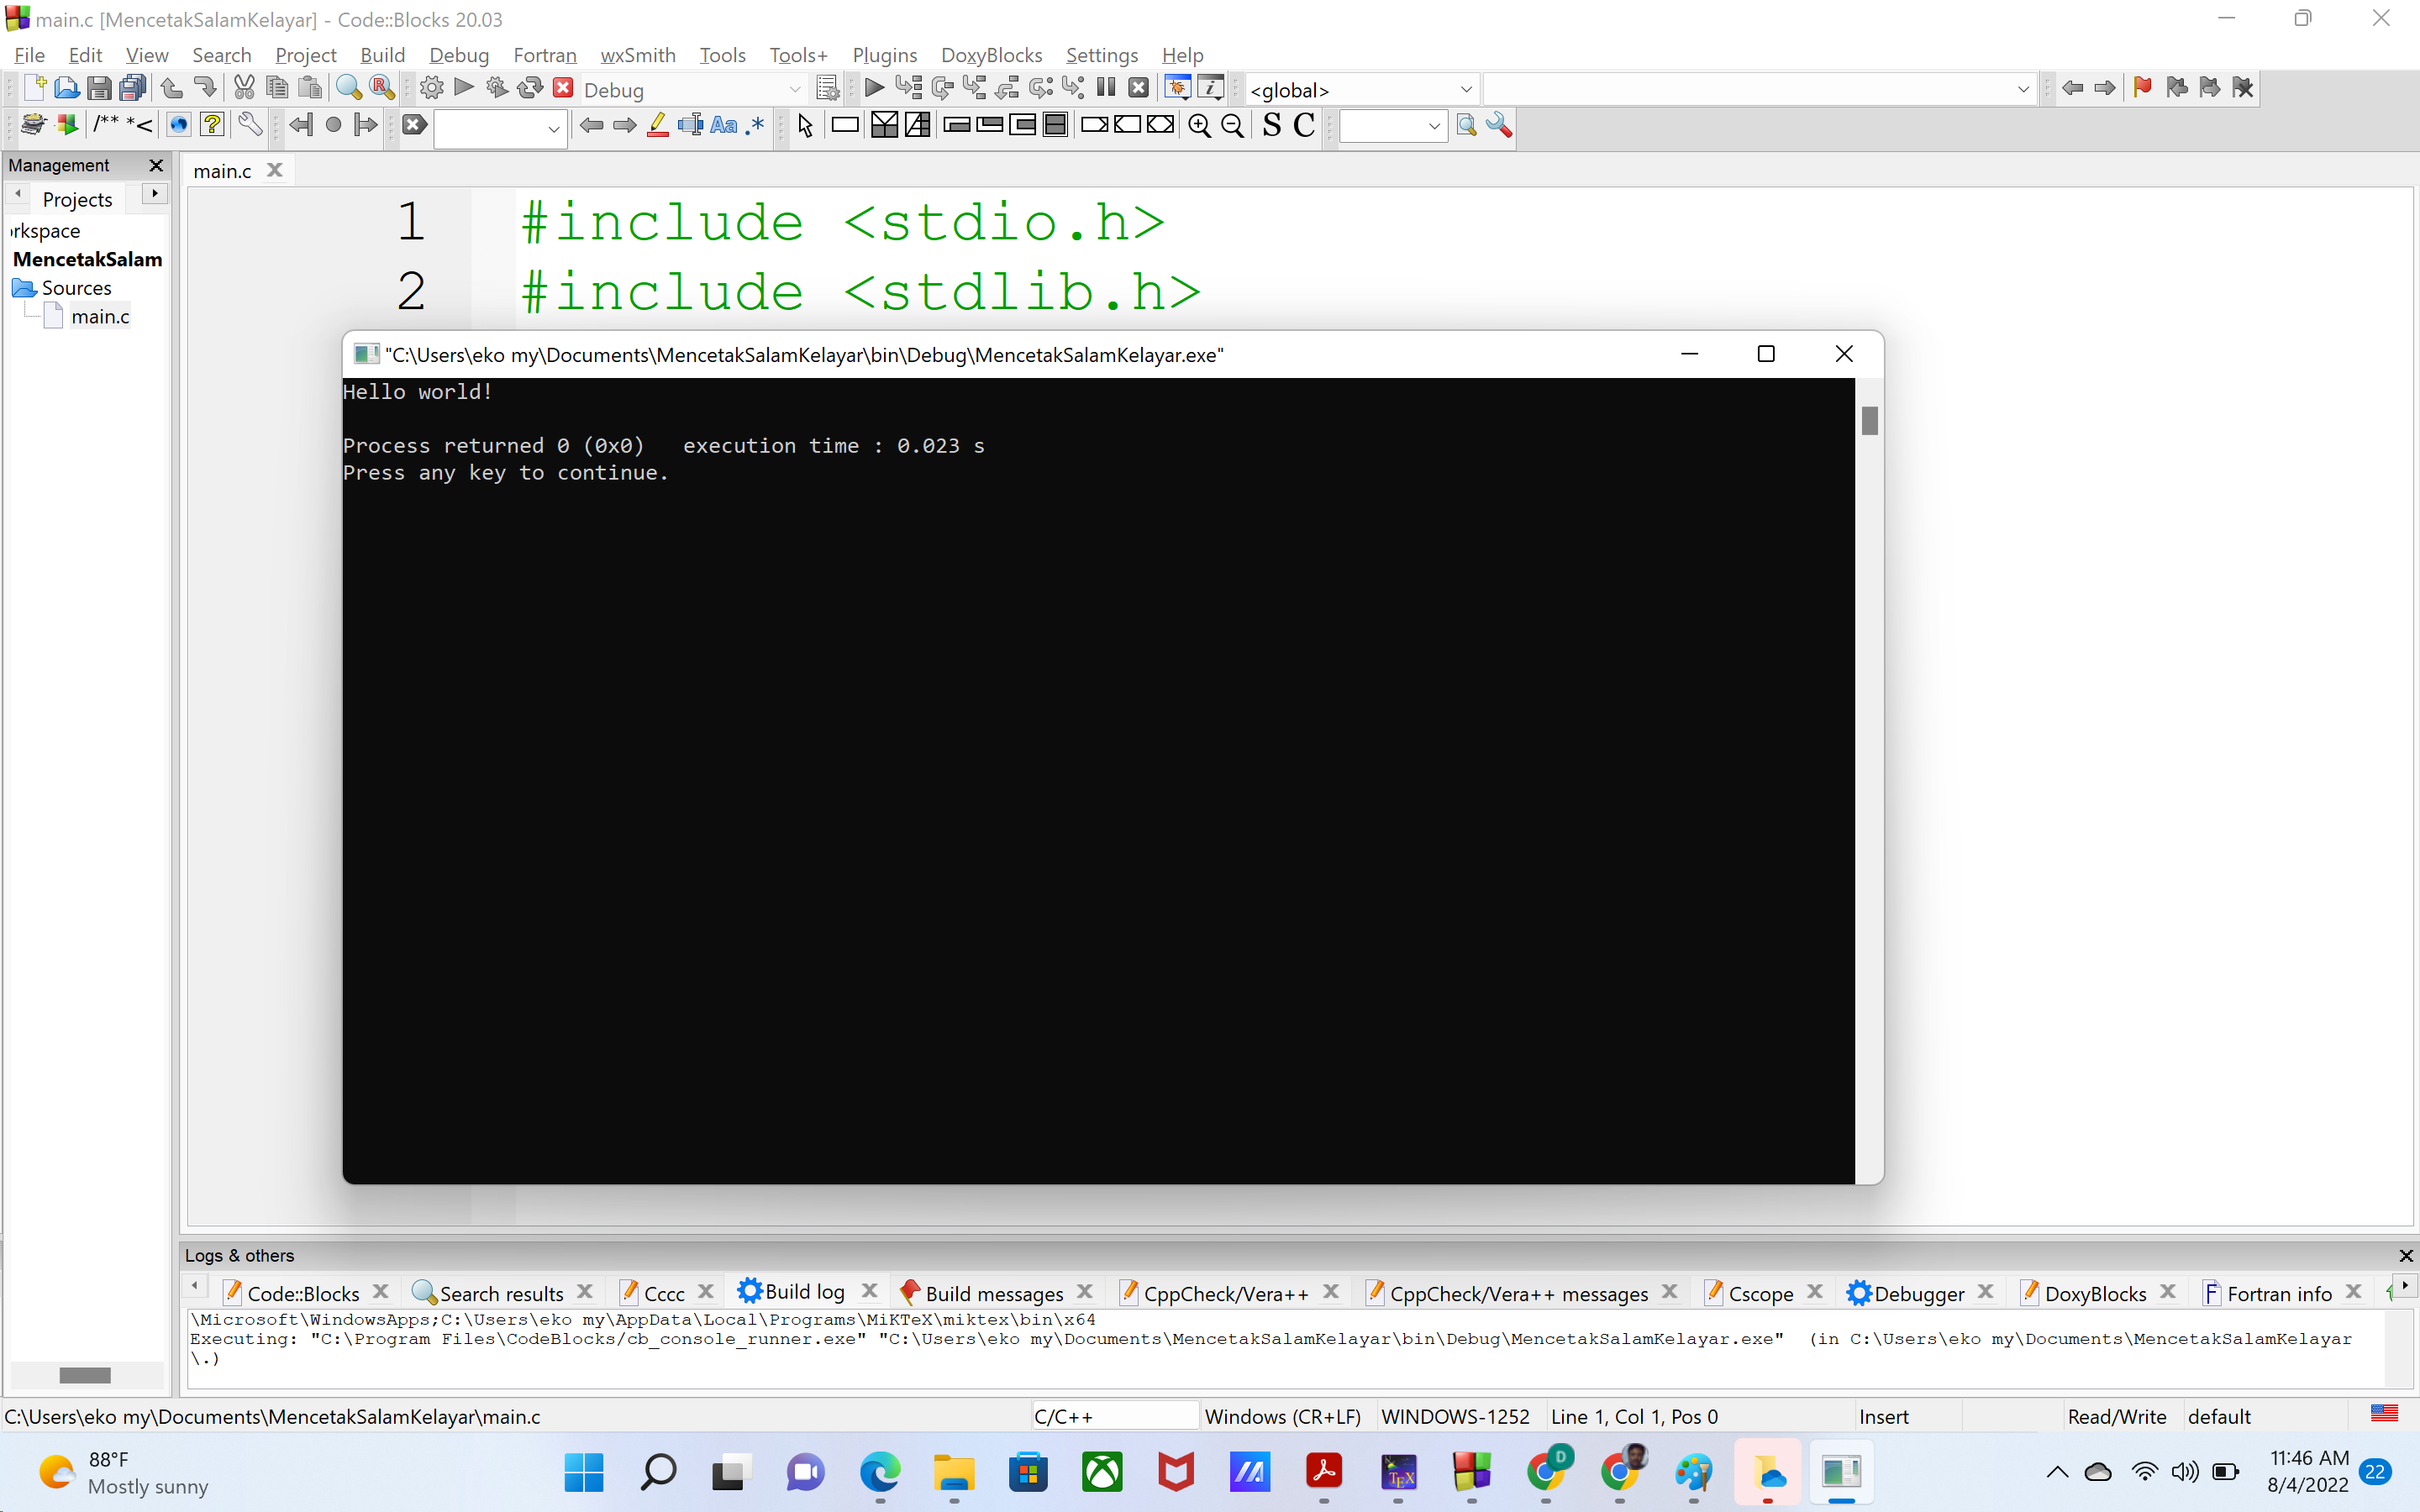
\includegraphics[width=0.7\linewidth]{P1/img/screenshot010.png}
		      \caption{}
		      \label{fig:screenshot010}
	      \end{figure}
\end{enumerate}

\section{Struktur Bahasa C}

\begin{lstlisting}[language=c,caption=Contoh program sederhana dalam bahasa C,label=lst:helloworld,captionpos=t]
	#include <stdio.h>

	int main() {
		printf("Hello World!");
		return 0;
	}
	\end{lstlisting}
Berikut adalah penjelasan kode di atas:
\begin{enumerate}
	\item \verb|#include <stdio.h>|
	merupakan sebuah header dimana kita memasukkan fungsi-fungsi yang ada di dalam file 'stdio.h' yang berisi fungsi input dan output dasar, seperti printf()
	\item int main()
    merupakan fungsi utama. fungsi ini pasti ada di setiap program bahasa C. 
    semua program yang ada di dalam kurung kurawal {} akan dieksekusi ketika program dijalankan.
	\item printf("Hello World!");
    sebuah fungsi untuk mengeluarkan output "Hello Wolrd!".
    bisa diperhatikan di bagian akhir terdapat tanda titik koma ';'. setiap pernyataan (statement) dalam bahasa C selalu diakhiri oleh tanda koma
	\item return 0;
    sebuah pernyataan (statement) yang mengembalikan nilai ke fungsi main(), fungsi akan berakhir ketika dikembalikan.
    program yang ditulis dibawahnya, meskipun masih berada di dalam kurung kurawal akan di abaikan.
\end{enumerate}
Bahasa C mengabaikan spasi (whitespace), sehingga program di atas bisa juga ditulis sebagai:
\begin{lstlisting}[language=c]
	int main(){printf("Hello World!");return 0;}
\end{lstlisting}
tetapi jika ditulis seperti itu akan lebih sulit untuk dibaca.
sehingga lebih baik untuk menulis program dengan spasi dan di baris yang berbeda agar lebih mudah untuk dibaca.

\subsection*{Tugas Pendahuluan 1}
\begin{enumerate}
	\item Dari contoh di atas, apa yang terjadi jika \verb|#include <stdio.h>| dihapus?
  	\item Jika kode ditulis seperti di bawah ini, apa yang terjadi? kenapa hal itu bisa terjadi?
	\begin{lstlisting}[language=c]
	#include <stdio.h>

	int main() {
		return 0;
		printf("Hello World!");
	}
	\end{lstlisting}
\end{enumerate}

\section{Tipe Data}

Dalam bahasa C ada 3 tipe data dasar, yaitu int (integer), float, char (character).

\subsection{integer}

tipe data integer menyimpan data berupa bilangan bulat (tidak ada koma).\\
\begin{center}
	\captionof{table}{Tipe data integer \label{tab:integer}}
	\begin{tabular}{|l|c|l|}
		\hline
		\textbf{Tipe} & \textbf{Ukuran (byte)} & \textbf{Keterangan} \\
		\hline
		int 		& 4 		& tipe dasar integer \\
		short 		& 2 		& menyimpan integer yang lebih kecil \\
		long 		& 4 atau 8 	& menyimpan integer yang lebih besar, tergantung sistem \\
		long long 	& 8 		& bisa menampung angka sangat besar \\
		\hline
	\end{tabular}
\end{center}

\subsection{float}

tipe data float menyimpan data berupa bilangan desimal.
\begin{center}
	\captionof{table}{Tipe data float \label{tab:float}}
	\begin{tabular}{|l|c|l|}
		\hline
		\textbf{Tipe} & \textbf{Ukuran (byte)} & \textbf{Keterangan} \\
		\hline
		float 		& 4 	& tingkat ketelitian yang cukup untuk kebutuhan umum \\
		double 		& 8 	& ketelitian lebih tinggi, cocok untuk penghitungan ilmiah \\
		long double	& 10 	& ketelitian lebih tinggi dari double, tergantung pada compiler \\
		\hline
	\end{tabular}
\end{center}

\subsection{character}

tipe data ini menyimpan data berupa karakter, seperti sebuah huruf 'a', 'b', 'c', atau simbol '@', '\$', '?' dsb.
\begin{center}
	\captionof{table}{Tipe data char \label{tab:char}}
	\begin{tabular}{|l|c|l|}
		\hline
		\textbf{Tipe} & \textbf{Ukuran (byte)} & \textbf{Keterangan} \\
		\hline
		char & 1	& menyimpan kode ASCII. \\
		\hline
	\end{tabular}
\end{center}
ASCII (American Standard Code for Information Interchange) adalah standar kode karakter yang menghubungkan angka (0–127) dengan huruf, angka, tanda baca, dan simbol kontrol.
Dengan ASCII, komputer bisa menyimpan dan memproses teks karena setiap karakter punya kode numerik.

\subsection{Modifier}
Modifier adalah kata kunci tambahan di C yang dipakai untuk mengubah ukuran atau jangkauan nilai suatu tipe data dasar.
Modifier tidak bisa berdiri sendiri, harus digabung dengan tipe data dasar (int, char, dll).
Dalam bahasa C ada 4 modifier yaitu:
\begin{enumerate}
	\item signed \\
	modifier ini ada nilai default untuk int dan char. modifier ini hanya bisa digunakan untuk int dan char.
	dengan modifier ini sebuah tipe data bisa menyimpan nilai negatif dan positif.
    \\ contoh: \texttt{int a;}
	\item unsigned \\
    dengan modifier ini tipe data hanya menyimpan nilai positif.
	\\ contoh: \texttt{unsigned int b;}
    \item short \\
    dengan modifier ini sebuah integer memiliki ukuran lebih kecil, biasanya menjadi 2 bytes.
    \\ contoh: \texttt{short int c;} 
	\item long \\
    dengan modifier ini tipe data akan memiliki ukuran yang lebih besar.
	\\ contoh: \texttt{long int d;}
\end{enumerate}

\subsection*{Tugas Pendahuluan 2}
\begin{enumerate}
	\item Untuk menyimpan angka 2147483648, kita memerlukan tipe data apa? jelaskan!
	\item Jika kita ingin menyimpan nomor HP 12 digit (contoh: 012345678999), tipe data apa yang cocok untuk digunakan? jelaskan alasanmu!
\end{enumerate}


\section{Variabel}

Variabel merupakan sebuah tempat untuk menyimpan data.
Untuk menggunakan variabel, kita perlu mendeklarasikan variabel tersebut terlebih dahulu.
\\ Untuk mendeklarasikan variabel bisa dilakukan dengan cara berikut:
\begin{lstlisting}
	tipe_data nama_variabel.
\end{lstlisting}
\begin{enumerate}[label={}, leftmargin=*]
	\item \verb|tipe_data| adalah tipe data yang ingin kita simpan dalam variabel tersebut (seperti int, float, yang dipelajari di sub bab sebelumnya).
	\item \verb|nama_variabel| adalah nama dari variabelnya.
\end{enumerate}
dalam membuat nama sebuah variabel terdapat aturan yang harus diikuti, yaitu:
\begin{enumerate}
	\item Nama variabel hanya boleh berisi huruf, angka, dan garis bawah (underscore).
	\item Nama variabel harus diawali dengan huruf atau garis bawah, tidak boleh diawali angka.
	\item Spasi tidak diperbolehkan di dalam nama variabel.
	\item Nama variabel tidak boleh berupa kata kunci (keyword) atau reserved word (kata kunci yang sudah ditentukan oleh standar bahasa pemrograman).
	\item Nama variabel harus unik dalam program.
\end{enumerate}
kita juga bisa mendeklarasikan banyak variabel yang memiliki tipe data yang sama dalam 1 baris saja.
contoh: \verb|tipe_data nama1, nama2, nama3;|

\subsection*{inisialisasi variabel}

inisialisasi adalah memberi nilai awal pada variabel saat variabel itu dibuat.
inisialisasi ini penting karena sebuah variabel ketika dideklarasikan akan berisi garbage value(bisa acak).
untuk inisialisasi kita hanya perlu memasukkan nilai ke variabel menggunakan operator "=".
{
\captionsetup[lstlisting]{labelformat=empty, justification=raggedright, singlelinecheck=false} %agar caption tanpa label dan di kiri
\begin{lstlisting}[language=c, caption={syntax}]
	tipe_data nama = nilai_variabel;
\end{lstlisting}
}
untuk mengubah nilai dari sebuah variabel kita bisa menggunakan cara yang sama seperti inisialisasi.
contoh:
\begin{lstlisting}[language=c]
	int a = 5; // inisialisasi variabel a bernilai 5
	a = 12; // nilai a berubah menjadi 12
\end{lstlisting}

\subsection*{Tugas Pendahuluan 3}
\begin{enumerate}
	\item perhatikan kode berikut:
	\begin{lstlisting}[language=c]
	int 2angka = 10;
	float tinggi-badan = 170,5;
	char nama lengkap = ' B ';
\end{lstlisting}
	kode di atas berisi deklarasi beberapa variabel.
	Sebutkan semua kesalahan yang ada pada kode tersebut dan jelaskan alasannya!
	Berikan contoh penulisan kode yang benar!
	\item perhatikan kode berikut:
	\begin{lstlisting}[language=c]
	const int a = 5;
	int b = 2;
	a++;
	b++;
\end{lstlisting}
	kode di atas terdapat sebuah error. Kenapa error tersebut terjadi? bagaimana cara memeperbaikinya?
\end{enumerate}

\section{Komentar}
komentar adalah sebuah baris atau bagian dari program yang diabaikan ketika dijalankan.
Komentar dapat digunakan untuk menjelaskan kode, dan membuatnya lebih mudah dibaca.
Komentar juga bisa digunakan untuk mencegah eksekusi kode saat melakukan pengujian.
\\ untuk menulis sebuah komentar dalam bahasa C, kita menggunakan double slash "//", semua hal yang ditulis setelah "//" dalam satu baris akan menjadi komentar.
contoh :
\begin{lstlisting}[language=c]
	//ini komentar
  	printf("halo dunia"); //ini juga komentar
	// printf("Kode di baris ini tidak akan berjalan");
\end{lstlisting}
komentar juga bisa ditulis dalam banyak baris dengan menggunakan "/*" dan "*/".
semua hal yang ditulis diantara "/*" dan "*/" akan menjadi komentar.
contoh:
\begin{lstlisting}[language=c]
/*
Contoh komentar
dengan banyak baris
*/
\end{lstlisting}

\subsection*{Tugas Pendahuluan 4}
\begin{enumerate}
	\item Perhatikan kode berikut:
	\begin{lstlisting}
	/*
		Ini adalah komentar
		/*
		komentar ini ada di dalam komentar
		*/
	*/
\end{lstlisting}
	Apakah penulisan komentar di atas benar? jika tidak, kenapa penulisannya salah?
	\item Untuk membuat komentar dengan banyak baris, kita bisa menggunakan tanda "/*" dan "*/".
	Apa yang terjadi jika hanya menggunakan tanda "/*" saja?
\end{enumerate}

\section{Operator}

Operator merupakan simbol yang merepresentasikan sebuah operasi yang dilakukan oleh sebuah atau beberapa nilai dan variabel.
nilai dan variabel yang digunakan dalam sebuah operasi disebut dengan operand.
\\ Dalam bahasa C, operator dibedakan menjadi 6 jenis berdasarkan fungsinya, yaitu:

\subsection{Operator Aritmatika}

digunakan untuk melakukan operasi aritmatika.
\begin{center}
	\captionof{table}{Operator Aritmatika\label{tab:aritmatika}}
	\begin{tabular}{|c|c|p{6cm}|c|}
		\hline
		\multicolumn{1}{|c|}{\textbf{Simbol}} &
		\multicolumn{1}{c|}{\textbf{Nama Operator}} &
		\multicolumn{1}{c|}{\textbf{Deskripsi}} &
		\multicolumn{1}{c|}{\textbf{Sintaks}} \\ \hline
		+   & Penjumlahan          & Menambahkan dua buah angka & a + b \\ \hline
		-   & Pengurangan          & Mengurangi angka pertama dengan angka kedua & a - b \\ \hline
		*   & Perkalian            & Mengalikan kedua angka & a * b \\ \hline
		/   & Pembagian            & Membagi angka pertama dengan angka kedua & a / b \\ \hline
		\%  & Modulus              & Menghasilkan sisa dari pembagian angka pertama dengan angka kedua & a \% b \\ \hline
		+   & Plus (unary)         & Menandakan sebuah angka merupakan bilangan positif & +a \\ \hline
		-   & Minus (unary)        & Menandakan sebuah angka merupakan bilangan negatif & -a \\ \hline
		++  & Increment            & Menambah nilai sebuah angka sebanyak 1 & a++ \\ \hline
		--  & Decrement            & Mengurangi nilai sebuah angka sebanyak 1 & a-- \\ \hline
	\end{tabular}
\end{center}


\subsection{Operator Relasional/Pembanding}

Digunakan untuk membandingkan dua operand.
Semua operator pembanding akan menghasilkan nilai true atau false sebagai hasil dari perbandingannya.
\begin{center}
	\captionof{table}{Operator Pembanding\label{tab:relasional}}
	\begin{tabular}{|c|p{3cm}|p{6cm}|c|}
		\hline
		\multicolumn{1}{|c|}{\textbf{Simbol}} &
		\multicolumn{1}{c|}{\textbf{Nama Operator}} &
		\multicolumn{1}{c|}{\textbf{Deskripsi}} &
		\multicolumn{1}{c|}{\textbf{Sintaks}} \\ \hline
		<   & Lebih kecil                & Bernilai benar jika operand kiri lebih kecil dari operand kanan & a < b \\ \hline
		>   & Lebih besar                & Bernilai benar jika operand kiri lebih besar dari operand kanan & a > b \\ \hline
		<=  & Lebih kecil atau sama dengan & Bernilai benar jika operand kiri lebih kecil atau sama dengan operand kanan & a <= b \\ \hline
		>=  & Lebih besar atau sama dengan & Bernilai benar jika operand kiri lebih besar atau sama dengan operand kanan & a >= b \\ \hline
		==  & Sama dengan                & Bernilai benar jika kedua operand bernilai sama & a == b \\ \hline
		!=  & Tidak sama dengan          & Bernilai benar jika kedua operand tidak sama & a != b \\ \hline
	\end{tabular}
\end{center}

\subsection{Operator Logika}

digunakan untuk menentukan logika antara kedua operand.
\begin{center}
	\captionof{table}{Operator Logika \label{tab:logic}}
	\begin{tabular}{|c|c|p{7cm}|c|}
		\hline
		\multicolumn{1}{|c|}{\textbf{Simbol}} &
		\multicolumn{1}{c|}{\textbf{Nama Operator}} &
		\multicolumn{1}{c|}{\textbf{Deskripsi}} &
		\multicolumn{1}{c|}{\textbf{Sintaks}} \\ \hline
		\texttt{\&\&} & Logika AND & Bernilai benar jika kedua operand bernilai benar & \texttt{a \&\& b} \\ \hline
		\texttt{||}   & Logika OR  & Bernilai benar jika salah satu atau kedua operand bernilai benar & \texttt{a || b} \\ \hline
		\texttt{!}    & Logika NOT & Bernilai benar jika operand bernilai salah & \texttt{!a} \\ \hline
	\end{tabular}
\end{center}

\subsection{Operator Bitwise}

Digunakan untuk melakukan operasi pada tingkat bit.
Operand akan diubah menjadi bilangan biner terlebih dahulu lalu baru dilakukan operasi pada operand tersebut.
\begin{center}
	\captionof{table}{Operator Bitwise \label{tab:bitwise}}
	\begin{tabular}{|c|l|p{8cm}|c|}
		\hline
		\multicolumn{1}{|c|}{\textbf{Simbol}} &
		\multicolumn{1}{c|}{\textbf{Nama Operator}} &
		\multicolumn{1}{c|}{\textbf{Deskripsi}} &
		\multicolumn{1}{c|}{\textbf{Sintaks}} \\ \hline
		\texttt{\&}  & Bitwise AND              & Melakukan operasi AND per bit dan mengembalikan hasilnya & \texttt{a \& b} \\ \hline
		\texttt{|}   & Bitwise OR               & Melakukan operasi OR per bit dan mengembalikan hasilnya & \texttt{a | b} \\ \hline
		\texttt{\^}  & Bitwise XOR              & Melakukan operasi XOR per bit dan mengembalikan hasilnya & \texttt{a \^ b} \\ \hline
		\texttt{\~}  & Bitwise NOT (Komplemen)  & Membalik semua bit (0 jadi 1, 1 jadi 0) & \texttt{\~a} \\ \hline
		\texttt{<<}  & Bitwise Left Shift       & Menggeser bit ke kiri sebanyak n posisi; ekuivalen dengan perkalian 2 tiap geseran & \texttt{a << b} \\ \hline
		\texttt{>>}  & Bitwise Right Shift      & Menggeser bit ke kanan sebanyak n posisi; ekuivalen dengan pembagian 2 tiap geseran & \texttt{a >> b} \\ \hline
	\end{tabular}
\end{center}

\subsection{Operator Penugasan (Assignment)}

Digunakan untuk emmberi nilai ke variabel.
\begin{center}
	\captionof{table}{Operator Assignment \label{tab:assignment}}
	\begin{tabular}{|c|l|p{8cm}|c|}
		\hline
		\multicolumn{1}{|c|}{\textbf{Simbol}} &
		\multicolumn{1}{c|}{\textbf{Nama Operator}} &
		\multicolumn{1}{c|}{\textbf{Deskripsi}} &
		\multicolumn{1}{c|}{\textbf{Sintaks}} \\ \hline
		=   & Assignment Sederhana & Memberikan nilai dari operand kanan ke operand kiri. & a = b \\ \hline
		+=  & Tambah dan Assign & Menjumlahkan operand kanan dengan operand kiri, lalu hasilnya disimpan ke operand kiri. & a += b \\ \hline
		-=  & Kurang dan Assign & Mengurangi operand kiri dengan operand kanan, lalu hasilnya disimpan ke operand kiri. & a -= b \\ \hline
		*=  & Kali dan Assign & Mengalikan operand kiri dengan operand kanan, lalu hasilnya disimpan ke operand kiri. & a *= b \\ \hline
		/=  & Bagi dan Assign & Membagi operand kiri dengan operand kanan, lalu hasilnya disimpan ke operand kiri. & a /= b \\ \hline
		\%=  & Modulus dan Assign & Mengambil sisa hasil bagi operand kiri dengan operand kanan, lalu hasilnya disimpan ke operand kiri. & a \%= b \\ \hline
		\&=  & AND Bitwise dan Assign & Melakukan operasi bitwise AND, lalu hasilnya disimpan ke operand kiri. & a \&= b \\ \hline
		|=  & OR Bitwise dan Assign & Melakukan operasi bitwise OR, lalu hasilnya disimpan ke operand kiri. & a |= b \\ \hline
		\verb|^=|  & XOR Bitwise dan Assign & Melakukan operasi bitwise XOR, lalu hasilnya disimpan ke operand kiri. & a \verb|^=| b \\ \hline
		>>= & Rightshift dan Assign & Menggeser bit operand kiri ke kanan, lalu hasilnya disimpan ke operand kiri. & a >>= b \\ \hline
		<<= & Leftshift dan Assign & Menggeser bit operand kiri ke kiri, lalu hasilnya disimpan ke operand kiri. & a <<= b \\ \hline
	\end{tabular}
\end{center}

\subsection{Operator Lainnya}

Selain operator di atas, dalam bahasa C terdapat operator lain yang digunakan untuk tugas spesifik.
Kita akan mendalami operator-operator ini pada modul berikutnya.
\begin{enumerate}
	\item \textbf{operator kondisional (?:)} \\
	ini adalah satu-satunya operator ternary (operator yang memiliki 3 buah operand) dalam bahasa C.
	digunakan untuk memeriksa suatu kondisi (pengganti if). \\
	contoh : \verb|kondisi ? hasil_jika_benar : hasil_jika_salah|
	\item \textbf{operator dot (.) dan arrow (->)} \\
	digunakan untuk mengakses member dalam struct \\
	\verb|structure_variable . member;| \\
	\verb|structure_pointer -> member;|
	\item \textbf{operator addressof (\&) dan Dereference (*)} \\
	operator '\&' mengembalikan nilai alamat dari sebuah variabel. \\
	contoh: \verb|&var| merupakan alamat dari variabel var \\
	operator '*' merupakan pointer kesebuah variabel. \\
	contoh: \verb|*var| merupakan pointer ke variabel var
\end{enumerate}

\subsection*{Tugas Pendahuluan 5}
\begin{enumerate}
	\item perhatikan kode berikut:
	\begin{lstlisting}[language=c]
	int a = 5;
	int b = 2;
	a += b += 3;
\end{lstlisting}
    Setelah kode tersebut dijalankan, berapa nilai a dan b? jelaskan langkah-langkahnya! jika ada error, jelaskan kenapa dan perbaiki kodenya!
	\item perhatikan kode berikut:
	\begin{lstlisting}[language=c]
	int m = 10, n = 3;
	int hasil = m / n;
\end{lstlisting}
    Setelah kode tersebut dijalankan, berapa nilai hasil? jelaskan langkah-langkahnya! jika ada error, jelaskan kenapa dan perbaiki kodenya!
  	\item perhatikan kode berikut:
  	\begin{lstlisting}[language=c]
	int m = 10, n = 3;
	int hasil = m / n += 2;
\end{lstlisting}
    Setelah kode tersebut dijalankan, berapa nilai hasil? jelaskan langkah-langkahnya! jika ada error, jelaskan kenapa dan perbaiki kodenya!
\end{enumerate}

\section{Output}

Dalam sub-bab syntax kita sudah mempelajari terkait printf("Hello World!");, fungsi printf() ini merupakan fungsi yang digunakan untuk mengeluarkan sebuah output ke terminal.
  Terminal adalah aplikasi untuk menjalankan perintah teks agar bisa berinteraksi dengan komputer, misalnya membuka folder, mengelola file, atau menjalankan program.
  fungsi printf() bisa kita tulis dengan Syntax
{
\captionsetup[lstlisting]{labelformat=empty, justification=raggedright, singlelinecheck=false} %agar caption tanpa label dan di kiri
\begin{lstlisting}[language=c, caption={syntax}]
	printf("format_string", variables/values);
\end{lstlisting}
}
\begin{enumerate}[label={}, leftmargin=*]
	\item formatted\_string : sebuah string yang akan dikeluarkan sebagai output, didalamnya bisa memiliki 'format specifier'
	\item variables/values : sebuah argument yang akan menggantikan format specifier yang ada dalam formatted\_string.
\end{enumerate}

\subsection{Format Specifier}
Format specifier adalah tanda khusus yang dipakai di dalam fungsi input/output (printf, scanf) untuk memberi tahu compiler tipe data apa yang akan ditampilkan atau dibaca.
Macam-macam format specifier:
\begin{center}
	\captionof{table}{Format Specifier dalam C \label{tab:format-specifier}}
	\begin{tabular}{|c|p{7cm}|c|}
		\hline
		\textbf{Specifier} & \textbf{Keterangan} & \textbf{Contoh Output} \\ \hline
		\%d   & integer (bilangan bulat) & 10 \\ \hline
		\%f   & float/double (bilangan pecahan) & 3.14 \\ \hline
		\%.2f  & 2 angka di belakang koma (angka 2 bisa diganti untuk mengatur jumlah angka di belakang koma) & 3.14 \\ \hline
		\%c   & char (karakter) & A \\ \hline
		\%s   & string (array of char) & Hello \\ \hline
		\%u   & unsigned integer & 25 \\ \hline
		\%o   & oktal & 017 \\ \hline
		\%x   & heksadesimal (huruf kecil) & 1a \\ \hline
		\%X   & heksadesimal (huruf besar) & 1A \\ \hline
		\%p   & alamat pointer & 0x7ffee \\ \hline
		\%\%  & tanda persen & \% \\ \hline
	\end{tabular}
\end{center}
Contoh:
\begin{lstlisting}[language=c]
#include <stdio.h>

int main() {
	int nrp = 5024991000;
	float ipk = 3.99;
	char grade = 'A';

	printf("Umur   : %d\n", nrp);	  // print output bilangan bulat
	printf("IPK    : %.2f\n", ipk);   // print output bilanghan desimal dengan 2 angka di belakang koma
	printf("Grade  : %c\n", grade);	  // print output karakter

	return 0;
}
\end{lstlisting}

\subsection{Escape Sequence}

Escape sequence adalah karakter khusus yang diawali dengan backslash (\textbackslash) dan dipakai di dalam string untuk mengontrol tampilan output.
\begin{center}
	\captionof{table}{Escape Sequence dalam C \label{tab:escape}}
	\begin{tabular}{|c|l|p{7.5cm}|}
		\hline
		\multicolumn{1}{|c|}{\textbf{Escape Sequence}} &
		\multicolumn{1}{c|}{\textbf{Nama}} &
		\multicolumn{1}{c|}{\textbf{Arti / Fungsi}} \\ \hline
		\textbackslash n   & Newline & Pindah ke baris baru \\ \hline
		\textbackslash t   & Horizontal Tab & Memberi jarak tab \\ \hline
		\textbackslash\textbackslash & Backslash & Menampilkan karakter backslash \textbackslash \\ \hline
		\textbackslash"   & Double Quote & Menampilkan tanda kutip ganda " \\ \hline
		\textbackslash'   & Single Quote & Menampilkan tanda kutip tunggal ' \\ \hline
		\textbackslash r   & Carriage Return & Kembali ke awal baris \\ \hline
		\textbackslash b   & Backspace & Menghapus 1 karakter sebelumnya \\ \hline
		\textbackslash f   & Form Feed & Pindah halaman (jarang dipakai) \\ \hline
		\textbackslash a   & Bell / Alert & Bunyi beep (tergantung sistem) \\ \hline
		\textbackslash 0   & Null Character & Penutup string di C \\ \hline
	\end{tabular}
\end{center}
Contoh:
\begin{lstlisting}[language=c]
#include <stdio.h>

int main() {
	printf("Hello\nWorld\n");         // baris baru
	printf("Nama:\tB300\n");          // tab
	printf("Kata hari ini: \"Bernafas\"\n"); // kutip ganda
	printf("C:\\Users\\Public\n");   // menampilkan path dengan \
	return 0;
}
\end{lstlisting}

\subsection*{Tugas Pendahuluan 6}
\begin{enumerate}
	\item Perhatikan kode berikut:
	\begin{lstlisting}[language=c]
	int main() {
		float a = 3.14;

		printf("%d", a);

		return 0;
	}
\end{lstlisting}
    Berapa nilai output yang ditampilkan? kenapa outputnya nilai itu? jika kita ingin outputnya itu "3.14", perubahan apa yang perlu dilakukan?
  	\item Buatlah sebuah program sederhana yang mengeluarkan output \verb|\'\'\'\'\'| !
\end{enumerate}

\section{Input}

dalam bahasa C, fungsi input yang sering digunakan adalah scanf().
scanf() bisa ditulis seperti berikut:
{
\captionsetup[lstlisting]{labelformat=empty, justification=raggedright, singlelinecheck=false} %agar caption tanpa label dan di kiri
\begin{lstlisting}[language=c, caption={syntax}]
	scanf("format", &var1, &var2, ...);
\end{lstlisting}
}
\begin{enumerate}[label={}, leftmargin=*]
	\item \verb|format|: sama seperti printf, ini berisi string dan juga format specifier.
\end{enumerate}
untuk variabel wajib menggunakan operator '\&' untuk mendapatkan alamat dari variabel.
\\ Contoh:
\begin{lstlisting}[language=c]
#include <stdio.h>

int main() {
	int umur;
	float ipk;
	char grade;

	// Input integer
	scanf("%d", &umur);

	// Input float
	scanf("%f", &ipk);

	// Input karakter
	scanf(" %c", &grade);

	// Output hasil input
	printf("\n=== Data ===\n");
	printf("Umur  : %d\n", umur);
	printf("IPK   : %.2f\n", ipk);
	printf("Grade : %c\n", grade);

	return 0;
}
\end{lstlisting}
\begin{verbatim}
	INPUT :
	21
	3.85
	A

	OUTPUT :
	=== Data ===
	Umur  : 21
	IPK   : 3.85
	Grade : A
\end{verbatim}
Dalam satu scanf() kita bisa mendapatkan banyak input untuk beberapa variabel.
Sehingga bagian scanf pada kode di atas bisa ditulis menjadi:
\begin{lstlisting}[language=c]
	// Input untuk ketiga variabel
	scanf("%d %f %c", &nrp, &ipk, &grade);
\end{lstlisting}

\subsection*{Tugas Pendahuluan 7}
\begin{enumerate}
	\item pada \verb|scanf("%d", &angka);| program meminta input integer untuk dimasukkan ke variabel angka.
     apa yang terjadi jika kita tulis \verb|scanf("%d", angka);| ? kenapa penulisan operator '\&' penting di scanf() ?
  	\item buatlah program sederhana yang menerima input dua angka integer lalu menampilkan hasil pembagian angka pertama dengan angka kedua di layar!
\end{enumerate}